\documentclass{mcmthesis}
 %\documentclass[CTeX = true]{mcmthesis}  % 当使用 CTeX 套装时请注释上一行使用该行的设置
\mcmsetup{tstyle=\color{black}\bfseries,%修改题号,队号的颜色和加粗显示,黑色可以修改为 black
        tcn = 25M656, problem = A, %修改队号,参赛题号
        sheet = true, titleinsheet = true, keywordsinsheet = true,%修改sheet显示信息
        titlepage = false, abstract = true}

        \usepackage{enumitem}
        \usepackage{tocloft} % 使用 tocloft 宏包
        \usepackage{setspace} % 允许调整行距
        
        % 调整目录标题之间的间距
        \setlength{\cftbeforesecskip}{2pt} % 调整 section 之间的距离(可改为实际需求长度)
        \setlength{\cftbeforesubsecskip}{2pt} % 调整 subsection 之间的距离
       % 调整 itemize 的行距和与正文的间距
        \setlist[itemize]{itemsep=2pt, topsep=3pt} % item 之间 5pt,itemize 与正文之间 10pt
        \setlength{\abovedisplayskip}{2pt}  % 全局调整公式上方间距
        \setlength{\belowdisplayskip}{2pt}  % 全局调整公式下方间距
        \setlength{\abovedisplayshortskip}{2pt}
        \setlength{\belowdisplayshortskip}{2pt}

        \usepackage{amsmath, amssymb, algorithm, algpseudocode, booktabs}



      %%%%%%%%%%%下面是关于references的
      \usepackage{cite} % 推荐使用,优化引用格式
      \usepackage{geometry}
      \geometry{left=1in, right=1in, top=1in, bottom=1in}
    % 调整引用为右上角标
    \makeatletter
    \def\@cite#1#2{\textsuperscript{[#1]}} % 设置右上角标格式
    \makeatother  
        
  %四款字体可以选择
  %\usepackage{times}
  \usepackage[scheme=plain]{ctex}%%%%%%%%%%%%%%%%%%%%%
  \usepackage{newtxtext,newtxmath} %CTeX 无此字体,可用 txfonts 替代,请使用新版 TeXLive.
  \usepackage[english]{babel} % 设置文档主要语言为英文%%%%%%%%%%%%%%%%%%%%
  %\usepackage{ctex}%%%%%%%%%%%%%%%%%%%%%%%%%%%%%%%%%%%%
  \usepackage{lastpage} % 获取总页数
 %\usepackage{palatino}
  %\usepackage{txfonts}
  \geometry{left=1in,right=0.75in,top=1in,bottom=1in}  % 设置1英寸的边距
\usepackage{indentfirst}  %首行缩进,注释掉,首行就不再缩进。
\usepackage{lipsum}
\usepackage{tikz}

\usepackage{enumitem} % 引入 enumitem 宏包
\usepackage{fontawesome5} % 加载 fontawesome5 宏包,用于指南针图标
\usepackage{amssymb} % 提供一些符号

\setlength{\parskip}{2pt}  % 设置段落间距为1个em
\setlength{\baselineskip}{1pt}  % 设置段内行距为1.5倍行高
\setlength{\textfloatsep}{3pt} % 图片与上下文之间的距离


\usetikzlibrary{shapes.geometric, arrows}
\usetikzlibrary{calc}
\graphicspath{{C:/Users/32624/Desktop/MCM/}}

\title{Neophocaena Asiaeorientalis in Vortex}
\author{\small \href{https://www.latexstudio.net/}
  {\includegraphics[width=7cm]{mcmthesis-logo}}}
\date{\today}

%%%%%%%%%%%%%%%%%%%%%%%%%%%%%%%%%%%%%%%%%(上面的部分你们不要动,有格式问题找ww)
\begin{document}
\begin{abstract}%这里是摘要部分
    \par       
\begin{keywords}%这里是关键词
               
\end{keywords}
\end{abstract}   

\maketitle
\newpage
\pagestyle{main}
\setcounter{page}{2} % 设置页码从 2 开始
\tableofcontents

\newpage
%正文
\section{Introduction}
\subsection{Problem Background}
Stairs are a common architectural element in our daily lives and an indispensable part of architectural history. From modern buildings to ancient temples and churches, stairs are often found and serve as records of human history. However, as time passes, the surface of stairs gradually develops uneven wear due to long-term use. These wears not only reflect how often and how the stairs were used, but also contain information about when they were built and the materials used, providing archaeologists with important clues about the history of the building.

Despite the important research value of stair wear, there are still relatively few targeted and systematic studies. Up to now, most analyses rely on qualitative observations and lack an analytical framework that can quantify wear patterns and their effects. To fill this research gap, there is an urgent need to develop mathematical models that combine the wear characteristics of stairs with information on foot traffic frequency, weight distribution, and environmental factors.

The wear traces of stairs exhibit complex and diverse patterns, combining these features, the goal of our article is to provide archaeologists with a feasible measurement method and quantitative analysis of stair wear by building a mathematical model to excavate the historical and cultural information in the wear of stairs.
\subsection{Restatement of the Problem}
The wear of stairs is a complex object of study influenced by multiple factors combined. By analyzing the background of the problem in depth and combining the specific constraints, the problem can be restated as follows:
\begin{itemize}
\item \textbf{Problem 1:}
Clarify the data requirements

Under the assumption that archaeologists can employ low-cost, simple, and non-destructive measurements, clarify the key types of data that need to be acquired.

\item \textbf{Problem 2:}
Build an analytical model

Build a mathematical model to analyze the wear of stairs and predict how the target stairs will be used, using the key data types acquired in Problem 1. Specifically include:
\hspace{2em} % 添加两个字符宽度的空格
\begin{flushleft}
A. The consistency between the wear patterns simulated by the model optimization and the actual wear patters of the staircase;

B. The direction in which the stairs are primarily used (upward or downward preference);

C. The number of people using the stairs simultaneously and their mode of use (e.g. side-by-side walking or single-passing).

\end{flushleft}

\item \textbf{Problem 3:}
Further exploration of issues related to specific conditions

Provided being able to estimate the age exists, clarifying the way the stairwell was used, and understanding the daily pattern of life in the structure, analyse the following aspects in depth:

\hspace{2em} % 添加两个字符宽度的空格
\begin{flushleft}
  
  D. Whether the wear patterns are consistent with the available information; 

  E. The estimation of the age of the stairs and its reliability;

  F. Identify the repairs and renovations conducted;

  G. The consistency between the material mechanical parameters used in the model and those obtained experimentally from the sources believed by archaeologists as the material origins;

  H. The information that can be determined includes the number of people using the stairs on a typical day and the usage frequency ( whether it involves a large number of people over a short time or a small number over a longer period).

\end{flushleft}
\end{itemize}

\subsection{Our Work}
\section{Assumptions and Justifications}
\begin{itemize}
\item \textbf{The materials from which the stairs are made have constant mechanical properties and for the same material, the mechanical properties are consistent throughout the stairs.}

\textbf{Explanation:}In practical scenarios, the internal variation of the material is minimal and can be disregarded, supporting the validity of this assumption.

\item \textbf{The effect of special shoes such as high-heeled shoes on the wear of stairs is not considered in the analysis, and only the role of common soles is investigated.}

\textbf{Explanation:}The wear effect of special shoes such as high-heeled shoes is usually concentrated in localized areas and happens less frequently, which has a modest influence on the overall wear pattern.

\item \textbf{The data obtained by the simulation expedition in the article is accurate and can truly reflect the wear of stairs and usage patterns.}

\textbf{Explanation:}Assumptions about the data that accurately reflect the wear of stairs and patterns of use will prevent data quality issues from interfering with the study.

\item \textbf{This study focuses on stone or wooden staircases that have been in use for a long time. It requires that the width of the stair treads be greater than the average foot length of Americans.}

\textbf{Explanation:}The problem statement explicitly specifies that the study is limited to stone or wooden stairs that show uneven wear after long-term use.

\item \textbf{All stair users walk at a normal gait , and the effects of intentional friction or other abnormal use behaviors on the wear of stairs are not considered.}

\textbf{Explanation:}Assuming that all stair users walk at a normal gait allows the study to focus on regular use and natural wear and tear, thus simplifying the model and avoiding the introduction of unnecessary complexity due to unusual behaviors(such as intentional rubbing or fast running).

\end{itemize}

Additionally, to simplify the analysis, additional assumptions were introduced and are discussed in the relevant sections.
\section{Notations}%可以有Definitions and Notations

Some important mathematical notations used in this paper are listed in Table 1:

\begin{table}[h!]
  \centering
  \caption{Notations and Definitions}
  \begin{tabular}{@{}lll@{}}
  \toprule
  \textbf{Symbol} & \textbf{Definition}                          & \textbf{Unit}              \\ \midrule
  \(W\)              & Wear volume                                  & cubic meters (m³)          \\
  \(R\)               & Wear rate                                    & cubic meters/second (m³/s) \\
  \(F_q\)              & Contact friction force                      & newtons (N)                \\
  \(F_G\)              & Vertical pressure                           & newtons (N)                \\
  \(CE\)              & Actual wear depth                           & meters (m)                 \\
  \(X\)               & Wear depth caused by friction               & meters (m)                 \\
  $\alpha $               & Wear depth caused by bending                & meters (m)                 \\
  \(K\)               & Number of people passing per unit time      & dimensionless              \\
  \(LEN\)             & Length of a single step                     & meters (m)                 \\
  \(WID\)             & Width of a single step                      & meters (m)                 \\
  \(HIG\)             & Height of a single step                     & meters (m)                 \\
  \(h\)               & Distance from the corresponding point to the lower tread    & meters (m)                 \\ \bottomrule
  \end{tabular}
  \end{table}

  \textbf{Note: Some variables are not listed here and will be explained in detail in the relevant sections.}
%wear amount
\section{Model Preparation}
\subsection{Guidance on Obtaining Information}
Before studying the wear of stairs, archaeologists must collect a variety of information about the target stairs to support subsequent modeling and analysis. This includes the following two components: measurement, literature search.



\begin{itemize}[label=$\diamond$]

\item \textbf{Measurement and data preprocessing of the depth of wear on stairs}

To ensure that the measurements are non-destructive, inexpensive, and can be done by a small number of people using minimal tools while maximizing the accuracy of the measurements, the following tools and measurement methods are chosen (Some of the tools can be referenced in Fig.1):

\begin{table}[h!]
  \caption{some Tools Used for Measurement and Their Benefits}
  \begin{tabular}{@{}lll@{}}
  \toprule
  \textbf{Name}          & \textbf{Function}                      & \textbf{Benefits}                \\ \midrule
  Laser Rangefinder      & Measures step depth and surface        & High accuracy, cost-effective     \\
                         & depressions                            & Facilitates data collection       \\
  Slide Rail             & Stabilizes laser rangefinder           & Ensures precise measurements      \\
                         & during movement                        &                                   \\
  Measuring Tape         & Measures basic dimensions              & Easy to use, low precision needs  \\
  Vernier Caliper        & Measures hard-to-reach areas           & Affordable, ensures completeness  \\
  D435                   & Modeling and visualization             & Partially visualizes measurements \\
  PC and Adapter Cable   & Used for data processing               &                                   \\ \bottomrule
  \end{tabular}
  \end{table}
  


\begin{figure}[h]  % 图片
  \small
  \centering  % 居中
  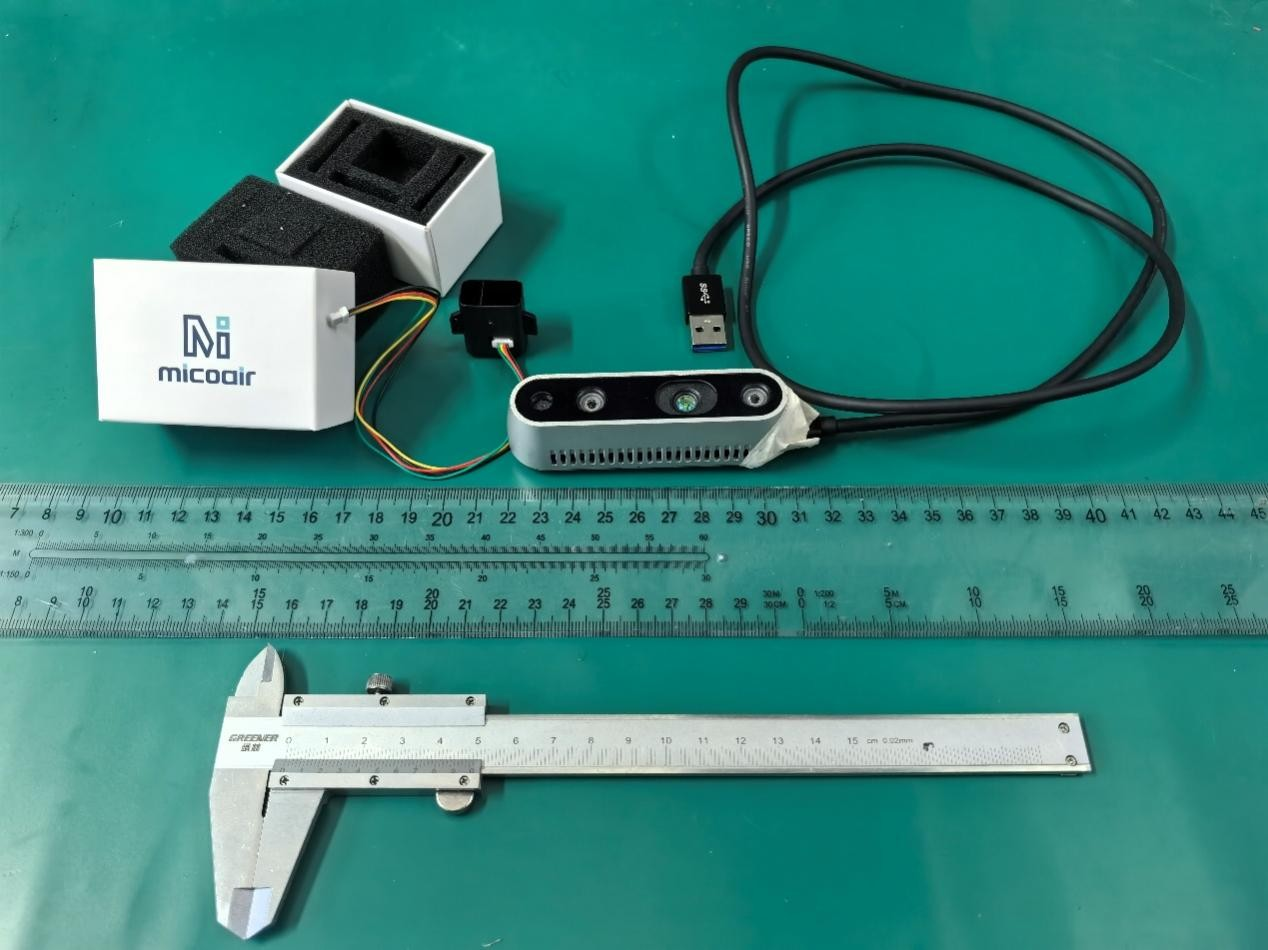
\includegraphics[width=12cm]{2-Measuring tools.jpg}
  \caption{Measuring tools} \label{fig:2}  % 标题与标签
  \end{figure}  % 图片结束



  Choose 20 steps of the target stairs and complete the following operations using the laser rangefinder and the vernier caliper for one steps:

\begin{enumerate}
\item Fix the laser range finder in a constant horizontal plane using a sliding table and set the height of the stair root as the reference height;

\item Randomly select 100 sample points for each square meter of the stair plane and record the 2D coordinates (x,y) of each sample point and its measured height.

\item Corners and other data that cannot be measured with a laser distance meter are measured with vernier calipers.

\end{enumerate}

Next, based on the data obtained from the measurements, we can use the following formula to calculate the depth of wear for each sampling point:

\[ CE = h_{\text{sampling point}} - h_{\text{reference}} \]

All the \(x, y, CE\) data from the sampling points will be integrated to construct the subsequent ideal staircase wear model.

\item \textbf{Step size measurement and data preprocessing}

Randomly select 10 steps from the target staircase and use a meter ruler to measure the length, width, and height of each step,record the data for each group and calculate the average to obtain the standard dimensions of the steps:

\[LEN_{\text{average}} = \frac{\sum_{i=1}^{10} LEN_i}{10}\]

\[\quad WID_{\text{average}} = \frac{\sum_{i=1}^{10} WID_i}{10}\]

\[\quad HIG_{\text{average}} = \frac{\sum_{i=1}^{10} HIG_i}{10}\]

\item \textbf{Data Retrieval from Literature and Sources}

The required information includes the construction period given by the archaeological team and the rough judgment on the types of materials made at the time of the inspection. Meanwhile, based on the rough judgment of the materials, query the data table and obtain the material mechanical parameters as shown in Table 2.


\begin{table}[h!]
  \centering
  \caption{Material Properties for Analysis}
  \label{tab:material_properties}
  \begin{tabular}{@{} p{8cm} c @{}}
  \toprule
  \textbf{Property} & \textbf{Symbol} \\
  \midrule
  Elastic Modulus & \( E \) \\
  Poisson Ratio & \( \nu \) \\
  Coefficient of Wear & \( k \) \\
  Material Hardness & \( H \) \\
  \bottomrule
  \end{tabular}
\end{table}

\end{itemize}
  
  

\subsection{Step Load Interaction Model}
To analyze the wear of stairs, it is essential to study how the force acts on the stairs when a person walks on them. Based on previous studies, we establish the Step Load Interaction Model (SLIM) to analyze the way forces act on stairs when a person walks on them. 
 



When a person walks on the stairs, the shoe is the only part that directly contacts the ground. Based on assumption 2, without considering footwear such as high-heeled shoes, which significantly change the way the force acts, and neglecting the mass of the shoe itself, we can consider the force of the shoe on the ground to be equivalent to the force of the foot on the shoe. That is, under this simplified condition, the shoe does not affect the magnitude and distribution of the force.  


\subsection{Step Load Interaction Model}
To analyze the wear of stairs, it is essential to study how the force acts on the stairs when a person walks on them. Based on previous studies, we establish the Step Load Interaction Model (SLIM) to analyze the way forces act on stairs when a person walks on them. 
 
\begin{figure}[h]  % 图片
  \small
  \centering  % 居中
  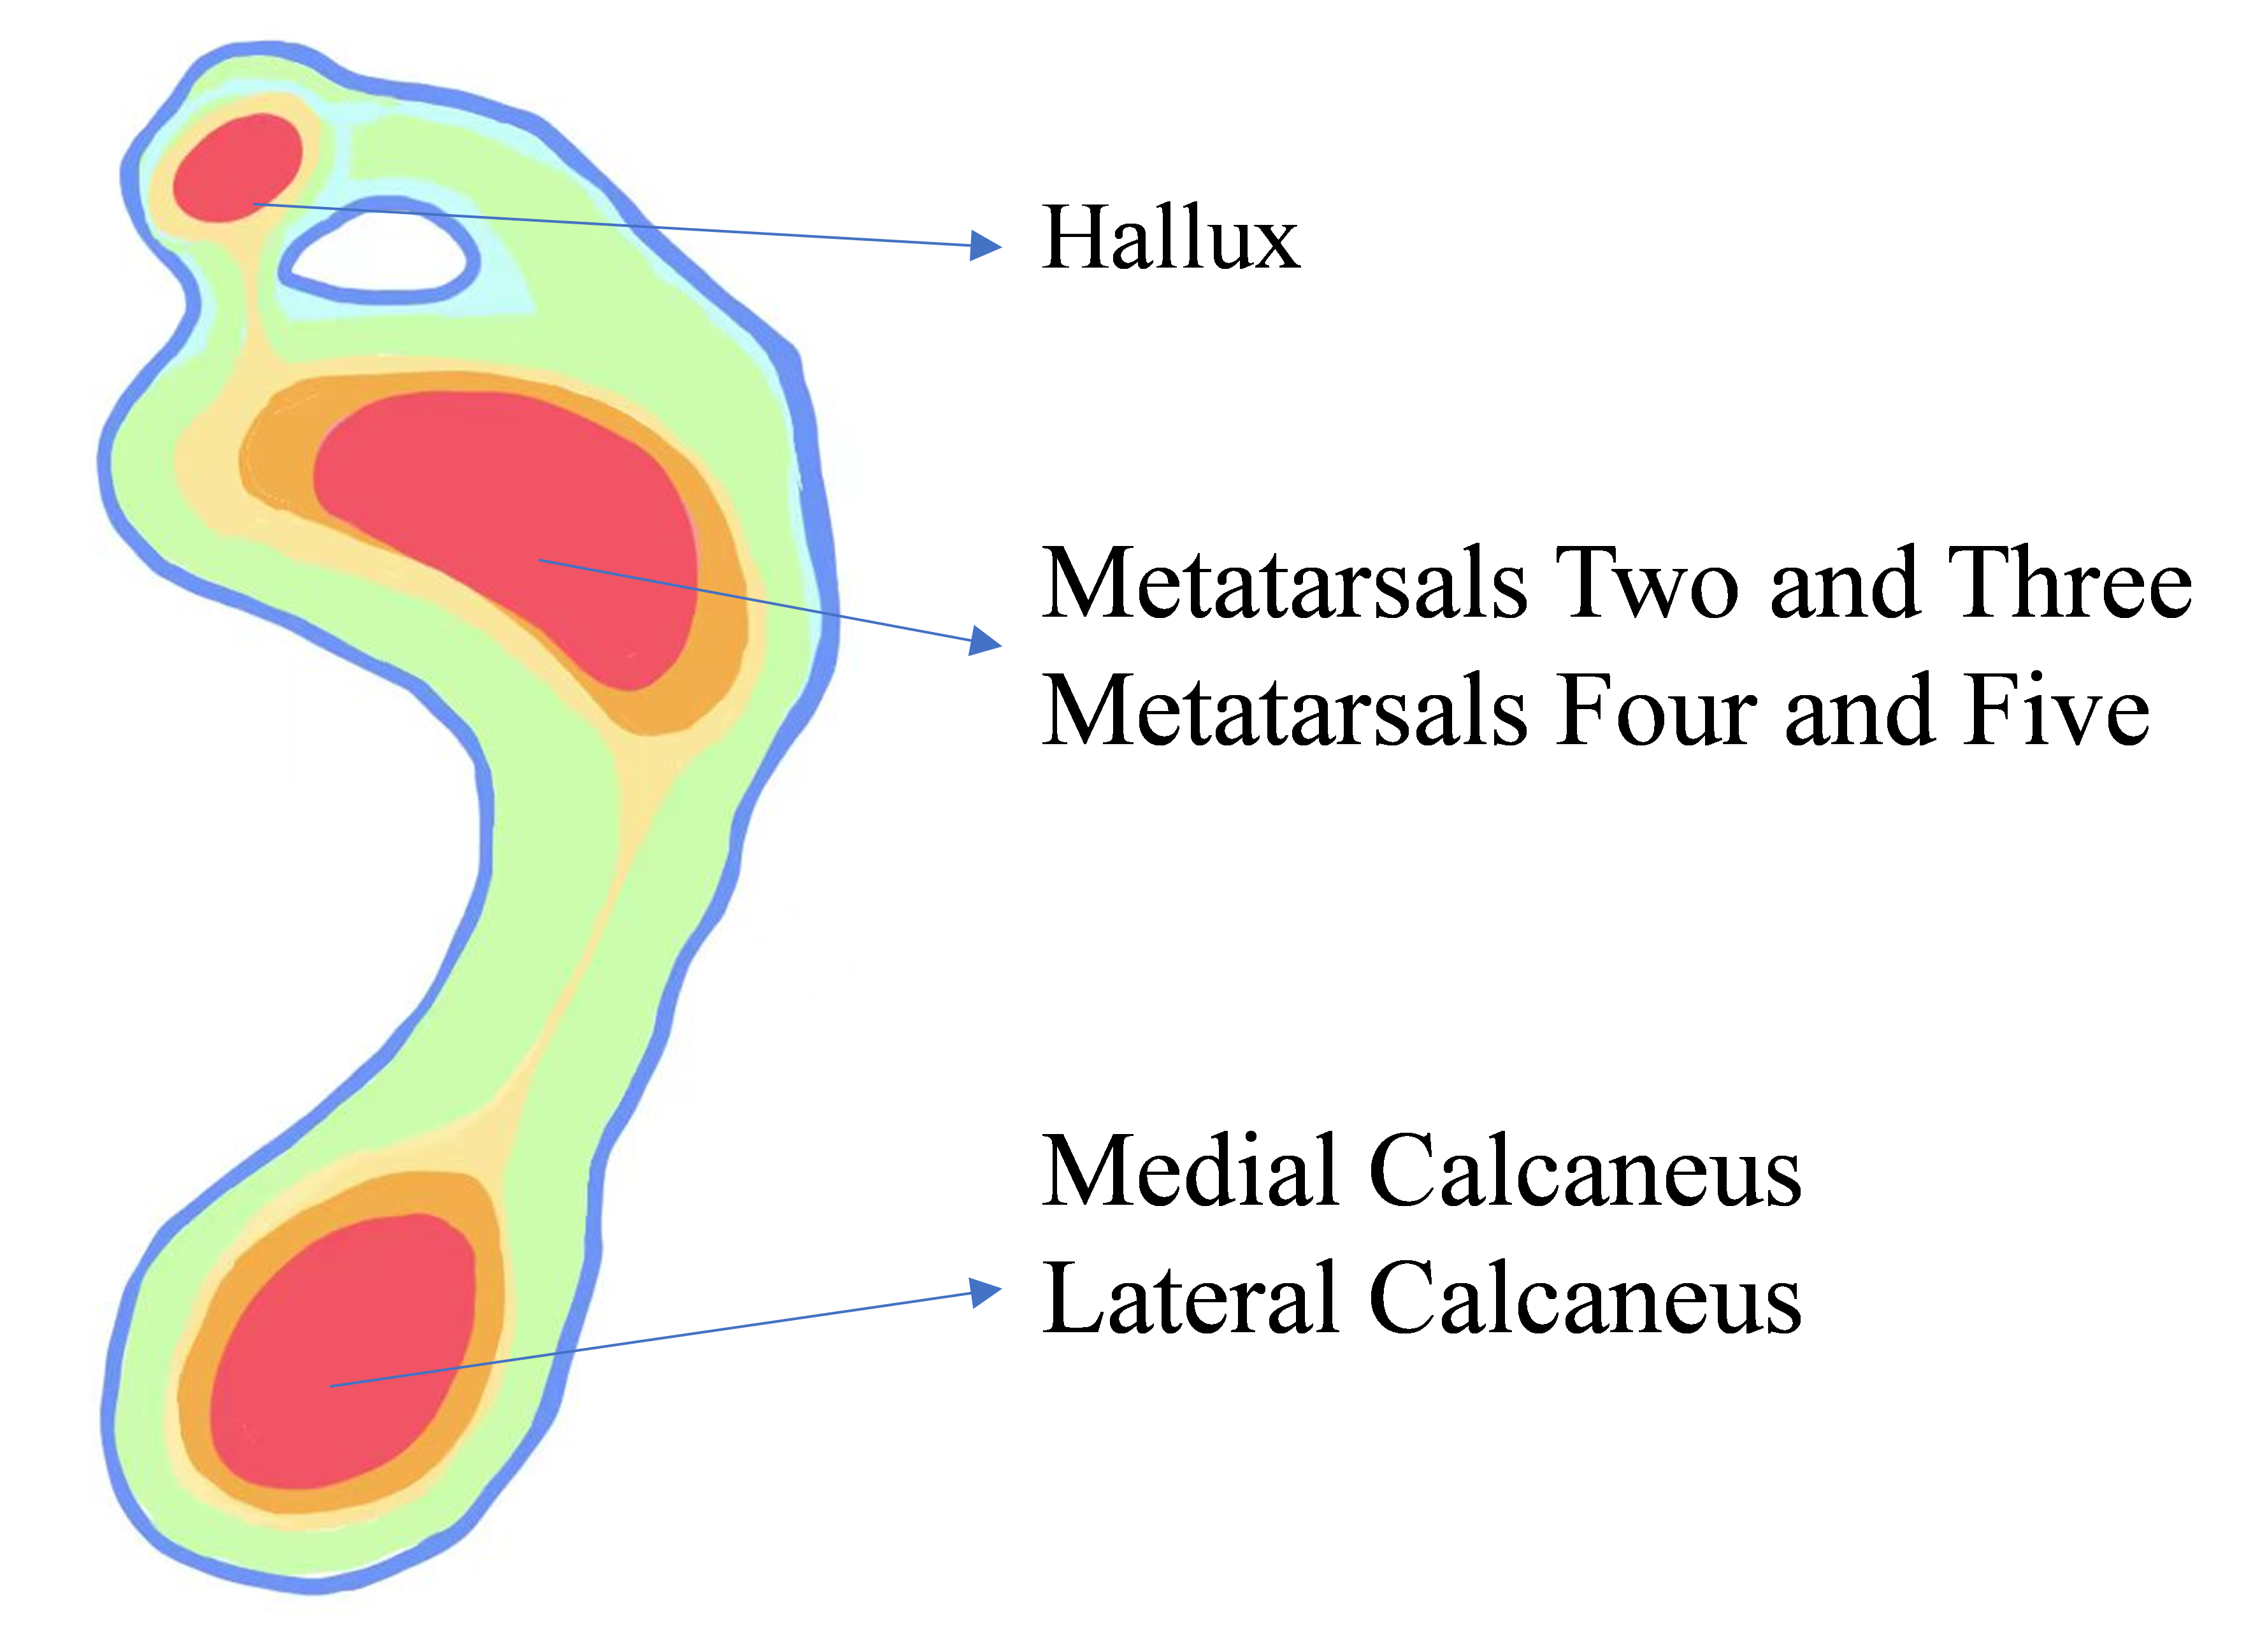
\includegraphics[width=10cm]{3-Infrared foot pressure zoning map.png}
  \caption{Infrared foot pressure zoning map} \label{fig:2}  % 标题与标签
  \end{figure}  % 图片结束




By reviewing the literature, we obtained an Infrared pressure distribution diagram of the force on the foot when a person is walking up and down stairs\cite{YISX202303023}(Fig.2). The blue part of this map indicates the minimum pressure and the orange and red parts indicate the maximum pressure. The parts with the highest pressure correspond to three parts of the foot, i.e. the Hallux region (first metatarsal), the Metatarsals two and three\& the Metatarsals four and five regions, as well as the Medical and Lateral Calcaneus regions, which are defined as the main force-bearing areas. To further study the area of the main force-bearing areas and its relationship with the total area of the foot, we first outlined the projection profile of the foot with a black line on the infrared distribution map. Subsequently, the grid method was used to process the images: when a certain grid was covered by one-half or more of the image area, it was counted as one grid, otherwise, it was ignored.  
%%%%%%%%%%%%%%%%%%%%%%%%%%%%%%%%%%%%%%%%%%%%%%%%%%%%%%%

\subsection{Step Load Interaction Model}
To analyze the wear of stairs, it is essential to study how the force acts on the stairs when a person walks on them. Based on previous studies, we establish the Step Load Interaction Model (SLIM) to analyze the way forces act on stairs when a person walks on them. 
 





Then, we counted 32 grids covered by the main force-bearing areas and 118 grids covered by the total projection of the foot, with the area share of the main stress portion being about 0.2712. Based on the average foot area of a U.S. citizen (approximately 245 cm\(^2\)), we calculat the average area of the main force-bearing areas to be 66.44 cm\(^2\), taking 66 cm\(^2\) to simplify the problem.

Thus, we can abstract the force of the foot on the stairs to the action of the main force area. According to the assumption 4,we can believe that when walking, the tips of the feet will not be in close contact with the inner edge of the stairs, the force exerted by a person walking on the stairs can be further simplified into the model shown in Figure n.
%%%%%%%%%%%%%%%%%%%%%%%%%%%%%%%%%%%%%%%%%%%%%%%%%%%%
Figure n shows that a countertop of stairs can be divided into two parts: the actual footprint section and the weathering section. To simplify the model, we assume that all stepping occurs in the actual footprint section and analyze the wear only in this section in the formal modeling.
\section{Synergizing Mechanics with Mathematical Modeling}
\subsection{Friction Model}
The Mills model is used to characterize the wear of materials under multiple loading conditions and is suitable for complex wear scenarios by considering the microscopic changes in the material surface and its elastic recovery properties.

In the case of stairs, which are used under stable conditions (e.g. constant flow of people and gait characteristics), the friction process is dominated by sliding wear due to the low sliding velocities. In this case, the contact state of the stair surface (including pressure and temperature distribution) remains stable during the friction process. Based on this assumption, the amount of wear W is usually linearly related to the nth power of the sliding velocity V, where n is the velocity factor, which is related to the material properties and contact conditions%%%%%%%%%%%%%%%%%%%%%%%%%%%%%%%%%网址的引用

On this basis, to more accurately analyze the wear behavior of staircase materials (e.g. stone or wood), we will modify the classical Mills model and develop a mathematical model suitable for staircase wear analysis.

First, the normal load F acting on the surface of the staircase material is calculated with the following expression:

\[ F(t) = \frac{F_{q} \cdot \mu}{1 + e^{t - \varepsilon }} \]

Where FG is the average value of normal pressure, $\varepsilon$  represents the adjustment coefficient, and μ represents the coefficient of kinetic friction.The F obtained above is used as an independent variable in the wear volume model to further calculate the material wear amount W:


\[ W = \int_{0}^{t} \frac{K \cdot V^{n} \cdot F(t)}{H} \ dt \]

Where V represents the average sliding velocity of the contact producing friction, and K and H are the wear coefficient and hardness of the staircase material, respectively.
\subsection{Bending Model}
To describe the wear behavior of stairs more accurately, a mathematical model based on beam bending theory is developed to predict the wear under different conditions through the relationship between deflection and loading.

\textbf{1.Variable description}
\begin{itemize}

\item \( \text{Wr} \): Deflection, the depth of deformation under external forces, measured in meters (m). 

\item \( \nu \): Poisson's ratio. 

\item \( k \): Shear correction factor. 

\item \( q \): Uniformly distributed load, measured in newtons per meter (N/m). 

\item \( E \): Elastic modulus, measured in pascals (Pa). 

\item \( I \): Moment of inertia of the stair cross-section, in meters to the fourth power (m\(^4\)). 

\item \( A \): Cross-sectional area of the stair, measured in square meters (m\(^2\)). 

\item \( g \): Gravitational acceleration, with a value of 9.98 meters per second squared (m/s\(^2\)). 

\item \( X \): Horizontal coordinate of the force application point, measured in meters (m). 



 \end{itemize}

\textbf{2.Coordinate axis description}

The coordinate axis of the stair adopts the left-handed rectangular coordinate system, the outer edge of the staircase coincides with the Y-axis, and the Z-axis is along the vertical direction of the stair, indicating the change of deformation and deflection, and the origin of the coordinate system is located at the bottom of the stair, as illustrated in the Figure 3.


\begin{figure}[h]  % 图片
  \small
  \centering  % 居中
  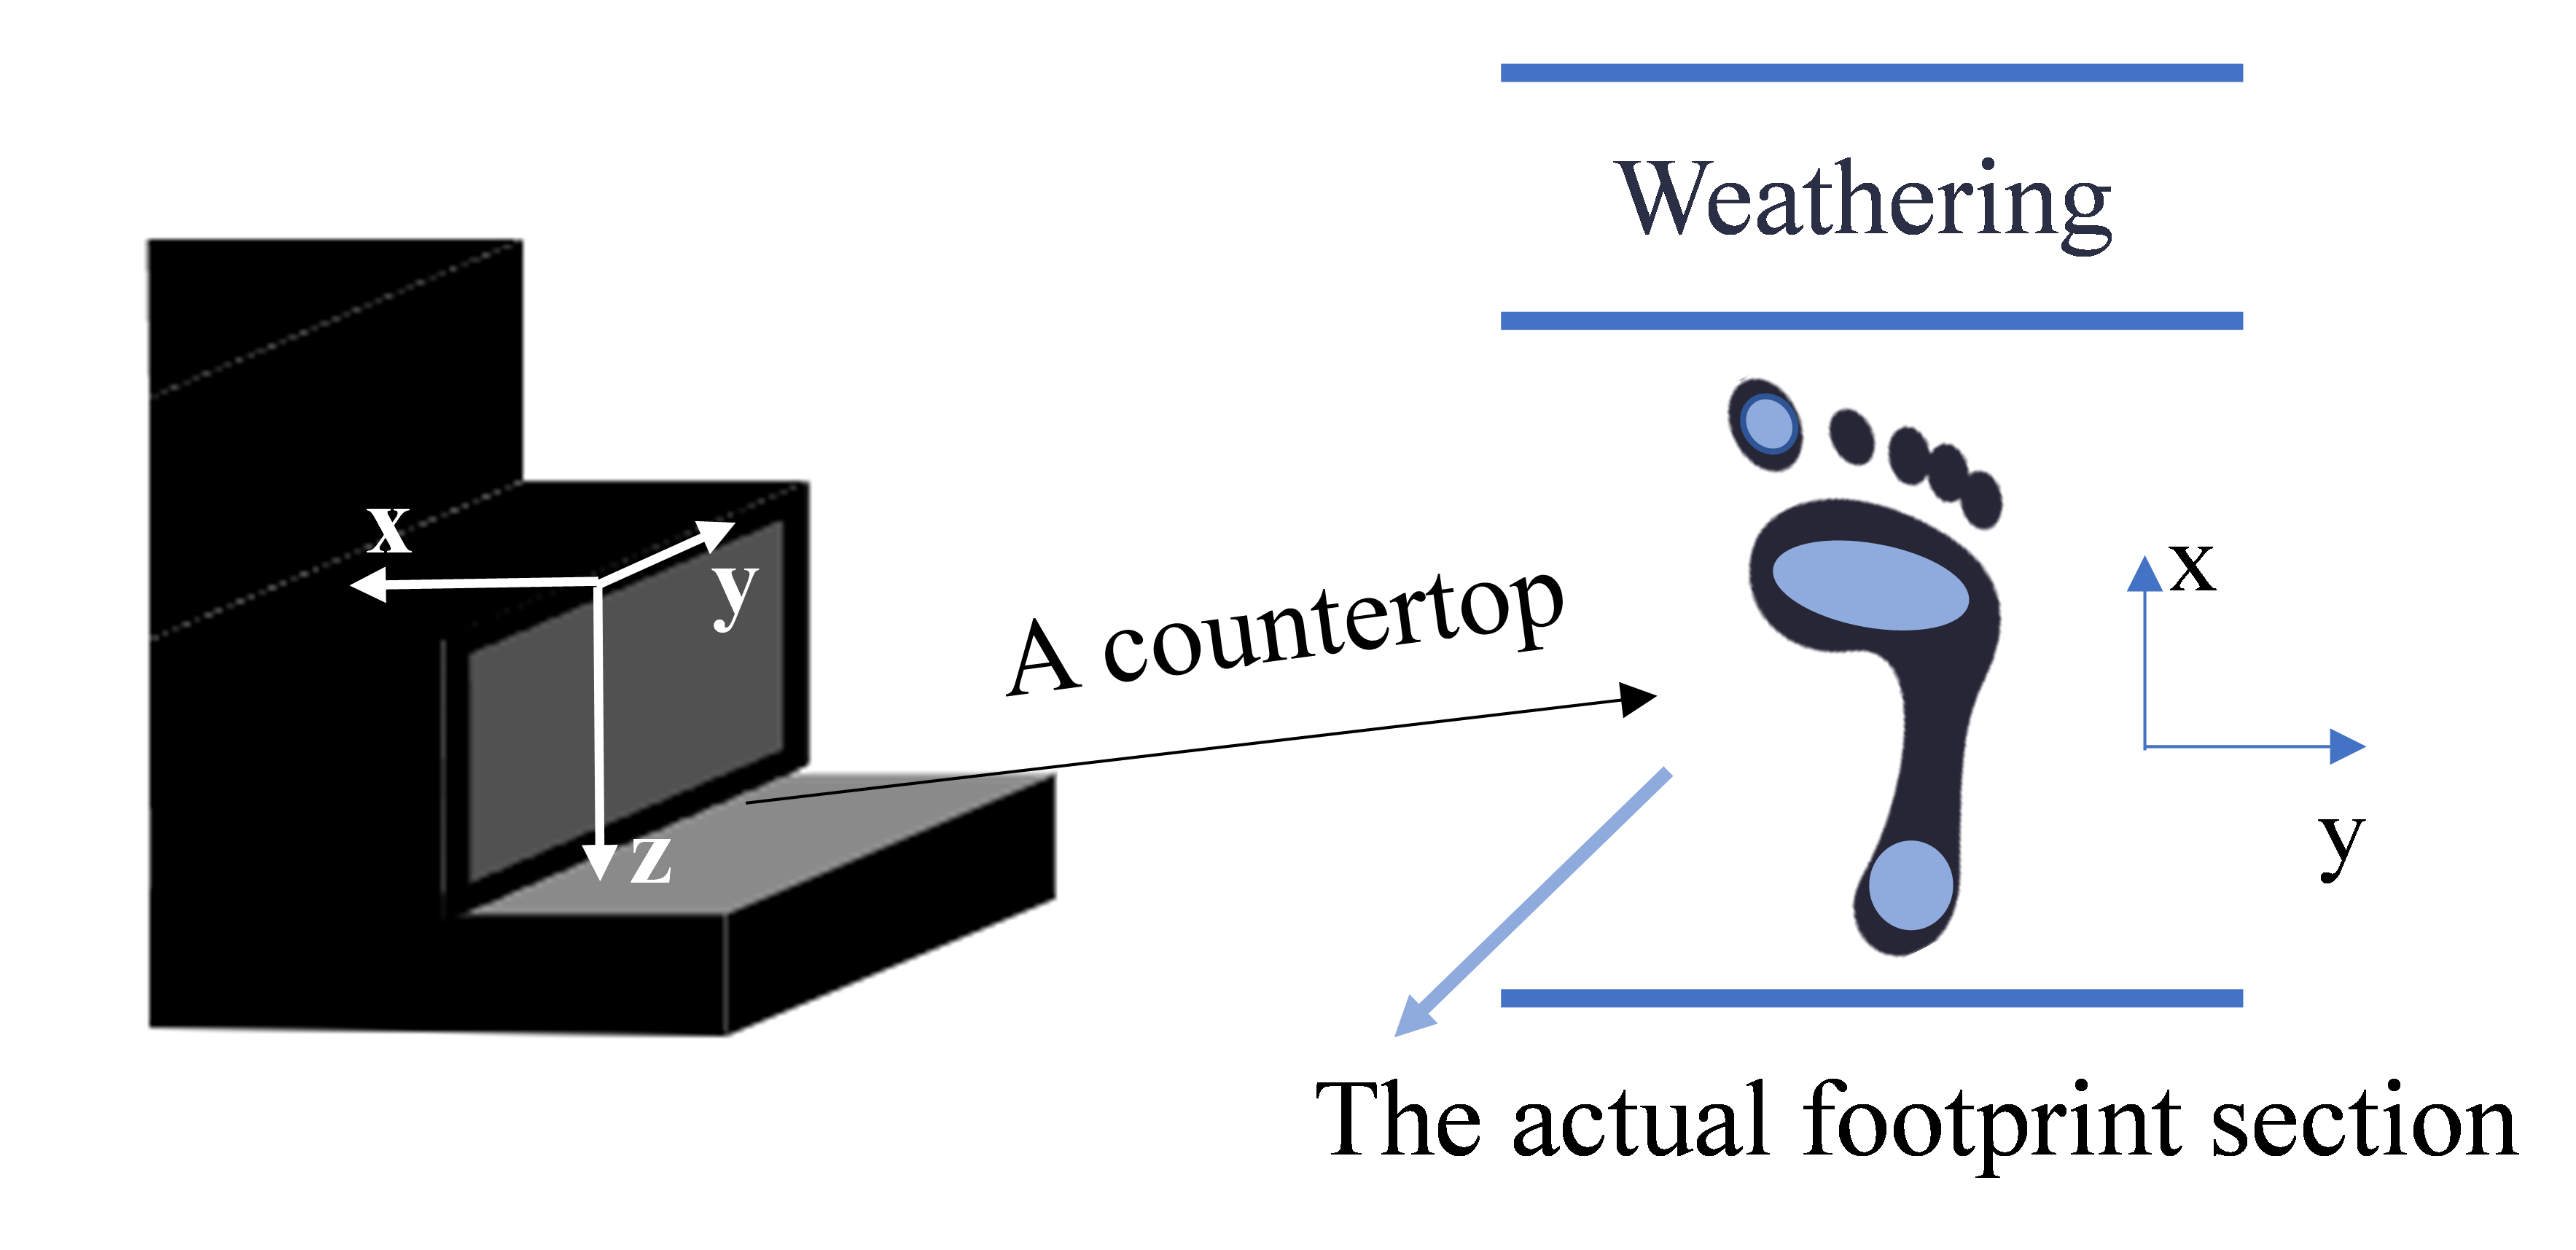
\includegraphics[width=10cm]{4-Establishment of stair coordinate axes and empirical partitioning of tread surfaces.png}
  \caption{Establishment of stair coordinate axes and empirical partitioning of tread surfaces} \label{fig:2}  % 标题与标签
  \end{figure}  % 图片结束




\textbf{3.model building}

Firstly, we simplify the stair to a model of a beam fixed at both ends (both ends are fixed by supports, one of which is supported with pulleys to allow sliding in the axial direction) \cite{Levinson1981}\cite{SJZT20241216003}. Based on this assumption, the deflection equation for this model is expressed as:

\[ W_r = \frac{9X}{24EI} \left[ X^3 - 2LEN \cdot X^2 + LEN^3 - \frac{12EI}{kgA}(X - LEN) \right] \]

From the above equation, We established the functional relationship between the deflection Wr and the horizontal coordinate of the force application point X and plotted the corresponding Figure 4. The Figure shows that the deflection reaches its maximum value near X=Xmax.

\begin{figure}[h]  % 图片
  \small
  \centering  % 居中
  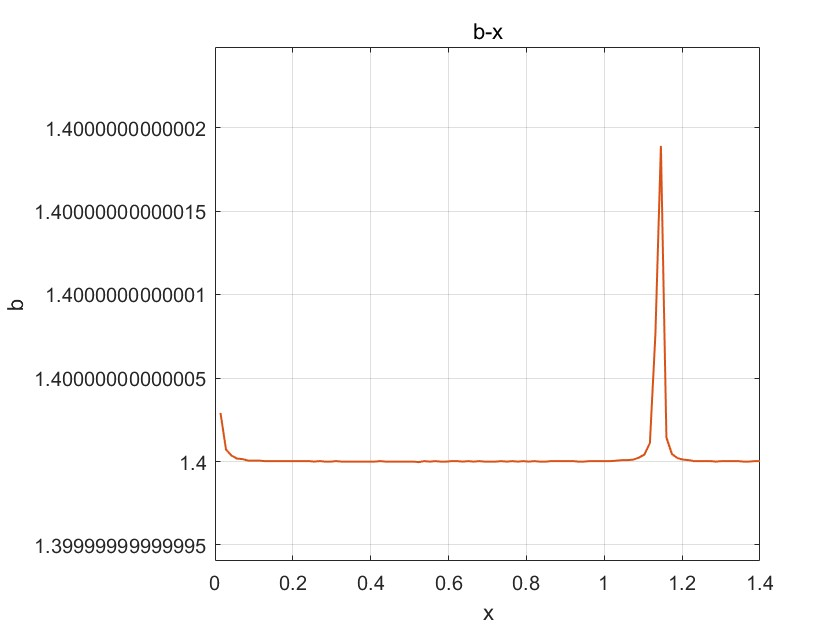
\includegraphics[width=10cm]{7-The depth of the depression on the staircase caused by the bending deformation.jpg}
  \caption{The depth of the depression on the staircase caused by the bending deformation} \label{fig:2}  % 标题与标签
  \end{figure}  % 图片结束








We further abstracted the overall bending deformation of the stairs as a concave region centered at Xmax, corresponding to the maximum deflection Wr. It is assumed that the cross-sectional profile of this region conforms to the shape of a catenary (while ignoring the deformation and concavity at other positions). The indentation caused by each normal load corresponds to the perimeter is calculated using the following equation:

\[ b = 2Wr \sinh\left(\frac{L_1}{2Wr}\right) \]

Where $L_1$ refers to The width corresponding to the indentation caused by each normal load.(b and $L1$ are specifically indicated in Figure 6)


\begin{figure}[h]  % 图片
  \small
  \centering  % 居中
  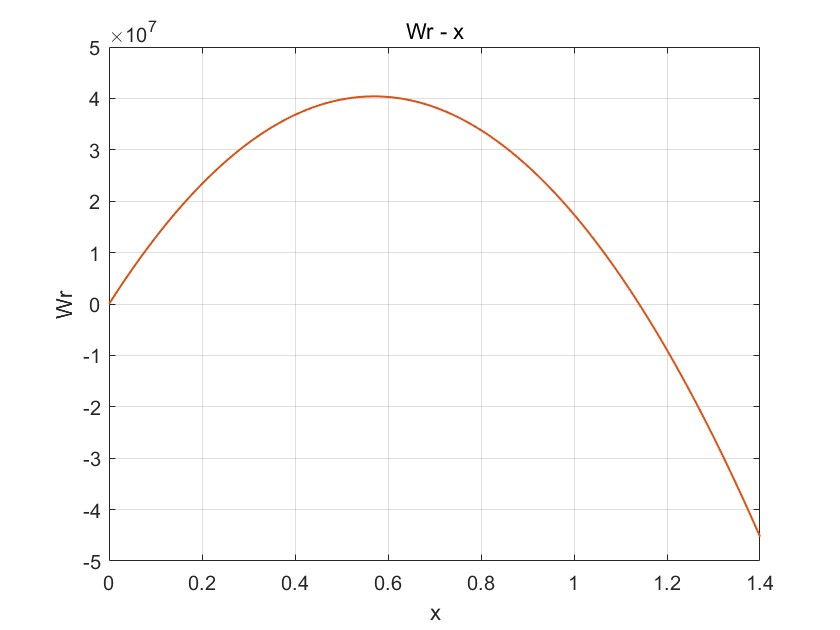
\includegraphics[width=9cm]{8-Length of catenary line-x.jpg}
  \caption{Length of catenary line} \label{fig:2}  % 标题与标签
  \end{figure}  % 图片结束


Through calculation, the wear width L1 caused by each applied load is determined to be 0.1±0.01. For the sake of simplification in subsequent calculations, L1 is treated as a constant value of 0.1.

\begin{figure}[h]  % 图片
  \small
  \centering  % 居中
  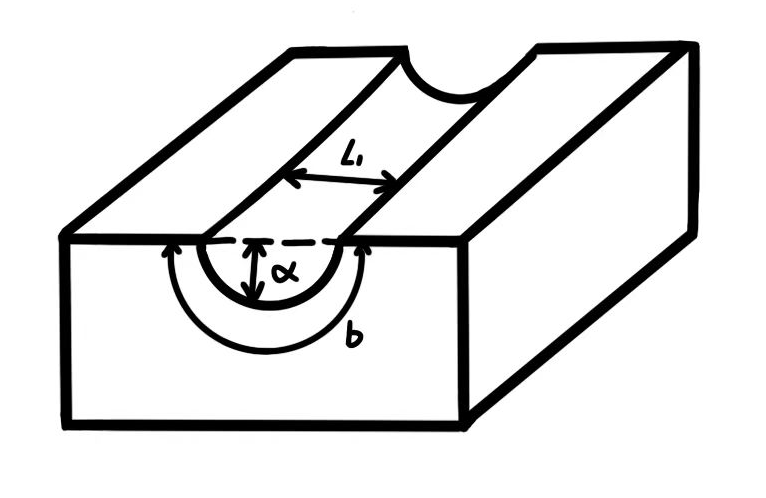
\includegraphics[width=9cm]{6-Bending model diagram.png}
  \caption{Bending model diagram} \label{fig:2}  % 标题与标签
  \end{figure}  % 图片结束

  \section{Step Load Interaction Model}
  To investigate the wear of stairs further, we first need to clarify the mechanical mechanism of human action on stairs during walking. To this end, this article developed the Step Load Interaction Model to quantify the distribution of each step's landing points during walking.
  
  \subsection{Model preparation}
  
  \begin{figure}[h]  % 图片
    \small
    \centering  % 居中
    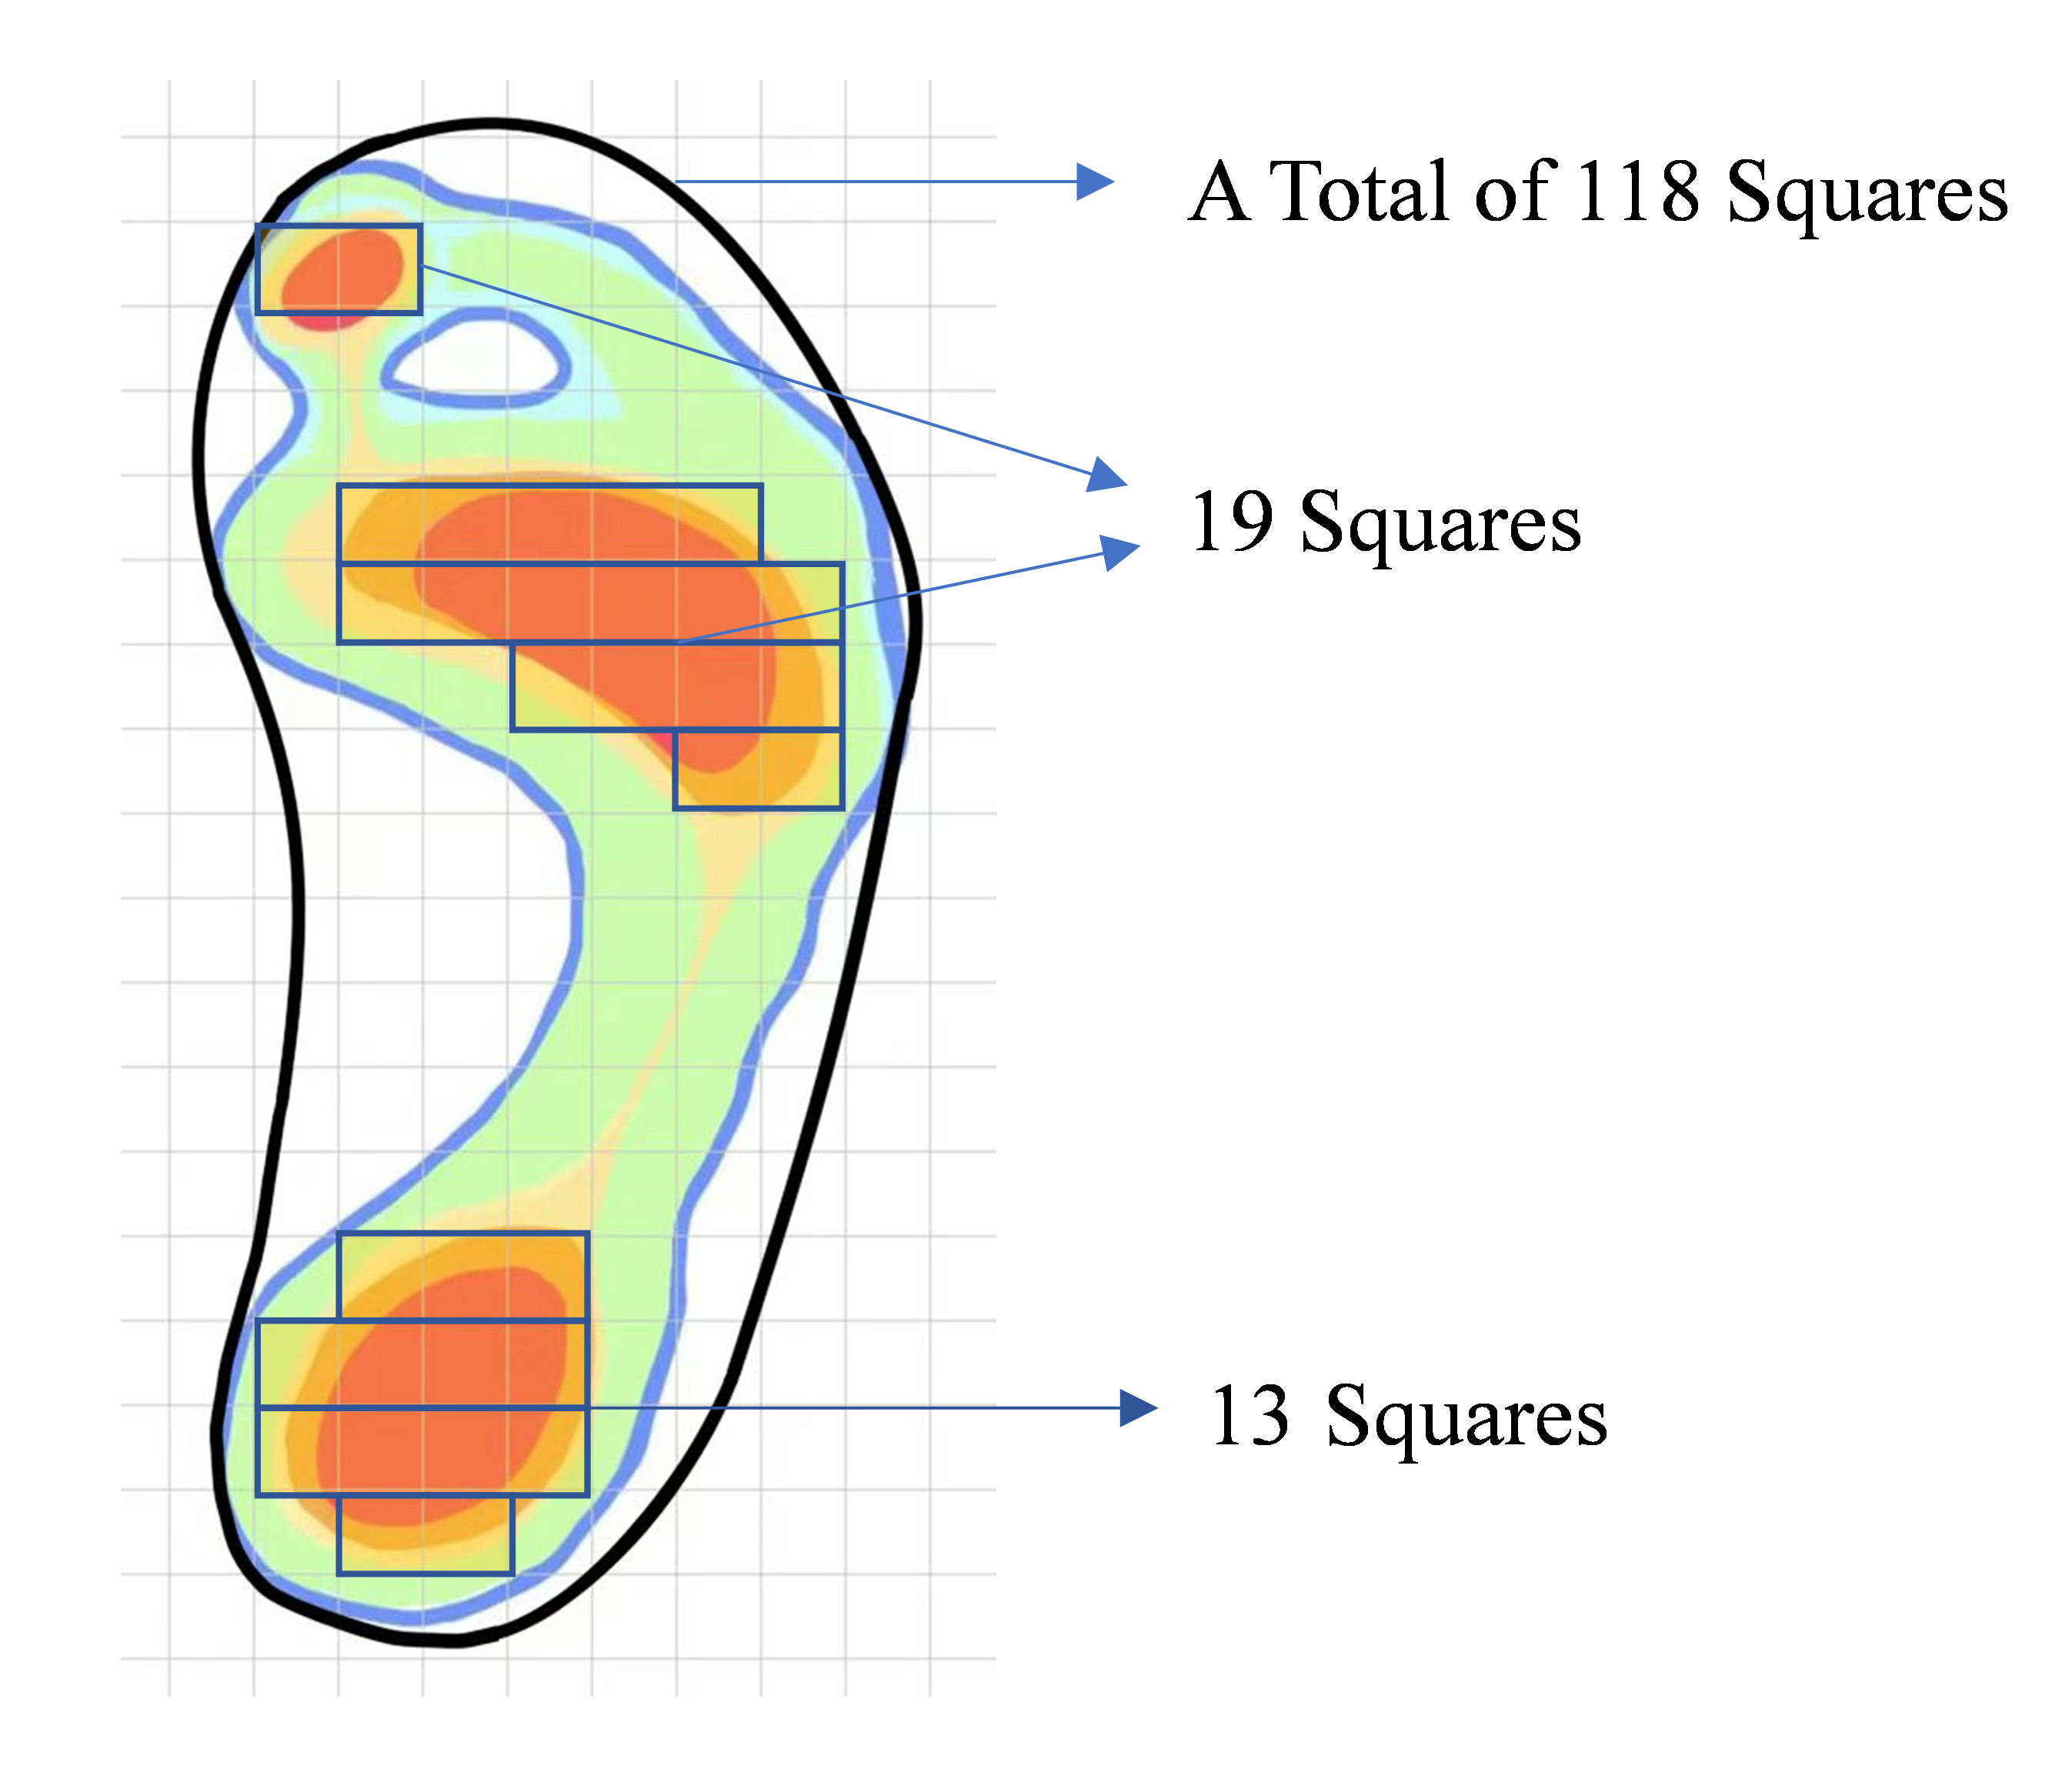
\includegraphics[width=10cm]{5-Foot sole grid.png}
    \caption{Foot sole grid} \label{fig:2}  % 标题与标签
    \end{figure}  % 图片结束
  
   Based on the FSCM, we have simplified the force exerted by a person walking on a stair. By analyzing the IR pressure distribution map using the grid method, the length and area of the foot as a whole and the three main force regions can be obtained as follows:
  
  \[
L_m = L_c = 54.44 \, \text{mm}, \quad L_h = 13.61 \, \text{mm}
\]
\[
S_m = 35 \, \text{mm}^2, \quad S_h = 4.15 \, \text{mm}^2, \quad S_c = 27 \, \text{mm}^2
\]
  
  
  Where \(L_i\) represents the length of region \(i\) and \(S_i\) refers to the area of region \(i\).
  
  Then, Take the x-axis of Figure 5 as the tread coordinate axis., According to relevant studies, the average width of the stair treads is about 32.5 cm and the height of staircase façade is about 14.5 cm \cite{WOS:000783553300001}
  
  Using half the length of the grid edge in Figure n as a unit of measurement, therefore, the width of the stair treads is about 48  \[D = 48\]
unit lengths and the height is about 21 unit lengths.
  
  To ensure that the landing point always remains within the countertop of the stairs, their range of values must satisfy the following constraints (due to space limitations, only the coordinate range of point M is presented here. The coordinate ranges for points U and C will be derived and explained in detail later based on the relationships among the three points):
  
  \begin{table}[h!]
    \centering
    \caption{Range of \(M\) Landing Coordinates}
    \begin{tabular}{@{}c cc@{}}
    \toprule
    \textbf{}      & \textbf{Forefoot Landing} & \textbf{Full Foot Landing} \\ \midrule
    \textbf{Ascending} & [0, 14]                  & [18, 30]                   \\ 
    \textbf{Descending} & \multicolumn{2}{c}{[4, 14]}                            \\ \bottomrule
    \end{tabular}
    \end{table}
  
  Where:
  
  \(U\): The pressure centers of Hallux  
  
  \(M\):The pressure centers of Metatarsals Two and Three Metatarsals Four and Five
  
  \(C\): The pressure centers of Medial Calcaneus Lateral Calcaneus 
  
  This section sets the geometric foundation for the subsequent analysis and provides a rational coordinate frame.
  
  
  \subsection{Walking patterns and Landing point analysis}
  
  In this model, it is assumed that a person walks up and down stairs in two ways and only two ways:
  
  \begin{itemize}
    \item Full-foot Walking: The entire foot applies force to the stairs.
  
    \item Forefoot Walking: Only the forefoot region applies force, while the rear foot remains suspended in the air.
  \end{itemize}
  
  
  In addition, each individual used only one walking style during a complete flight of stairs. To standardize the analysis, M is used as a benchmark.
  
  \begin{itemize}[label=$\diamond$]
  \item \textbf{Calculation of standard coordinates}
  \end{itemize}
  
  The standard coordinates on the i+1st step can be obtained recursively from the standard coordinates of the i-th step:
  
  \[
  X_n = X_n + L_{\text{stride}} - D
  \]
  
  
  Although walking styles vary, regardless of the style, the human stride length tends to keep the landing point of the next step within a “comfort zone”. When the expected landing point is outside the comfort zone, the walker adjusts the stride length to bring it back within a reasonable range. The comfort zone can be expressed as:
  
\[
\text{Full-foot Walking: } L_{\text{stride}} = [38, 58], \quad \text{Forefoot Walking: } L_{\text{stride}} = [36, 60]
\]


  On this basis, the standard coordinates of the i+1-th stair need to be adjusted according to the constraints of the comfort zone. The specific calculation process is shown in Figure 10. 
  
  
  \begin{figure}[h]  % 图片
    \small
    \centering  % 居中
    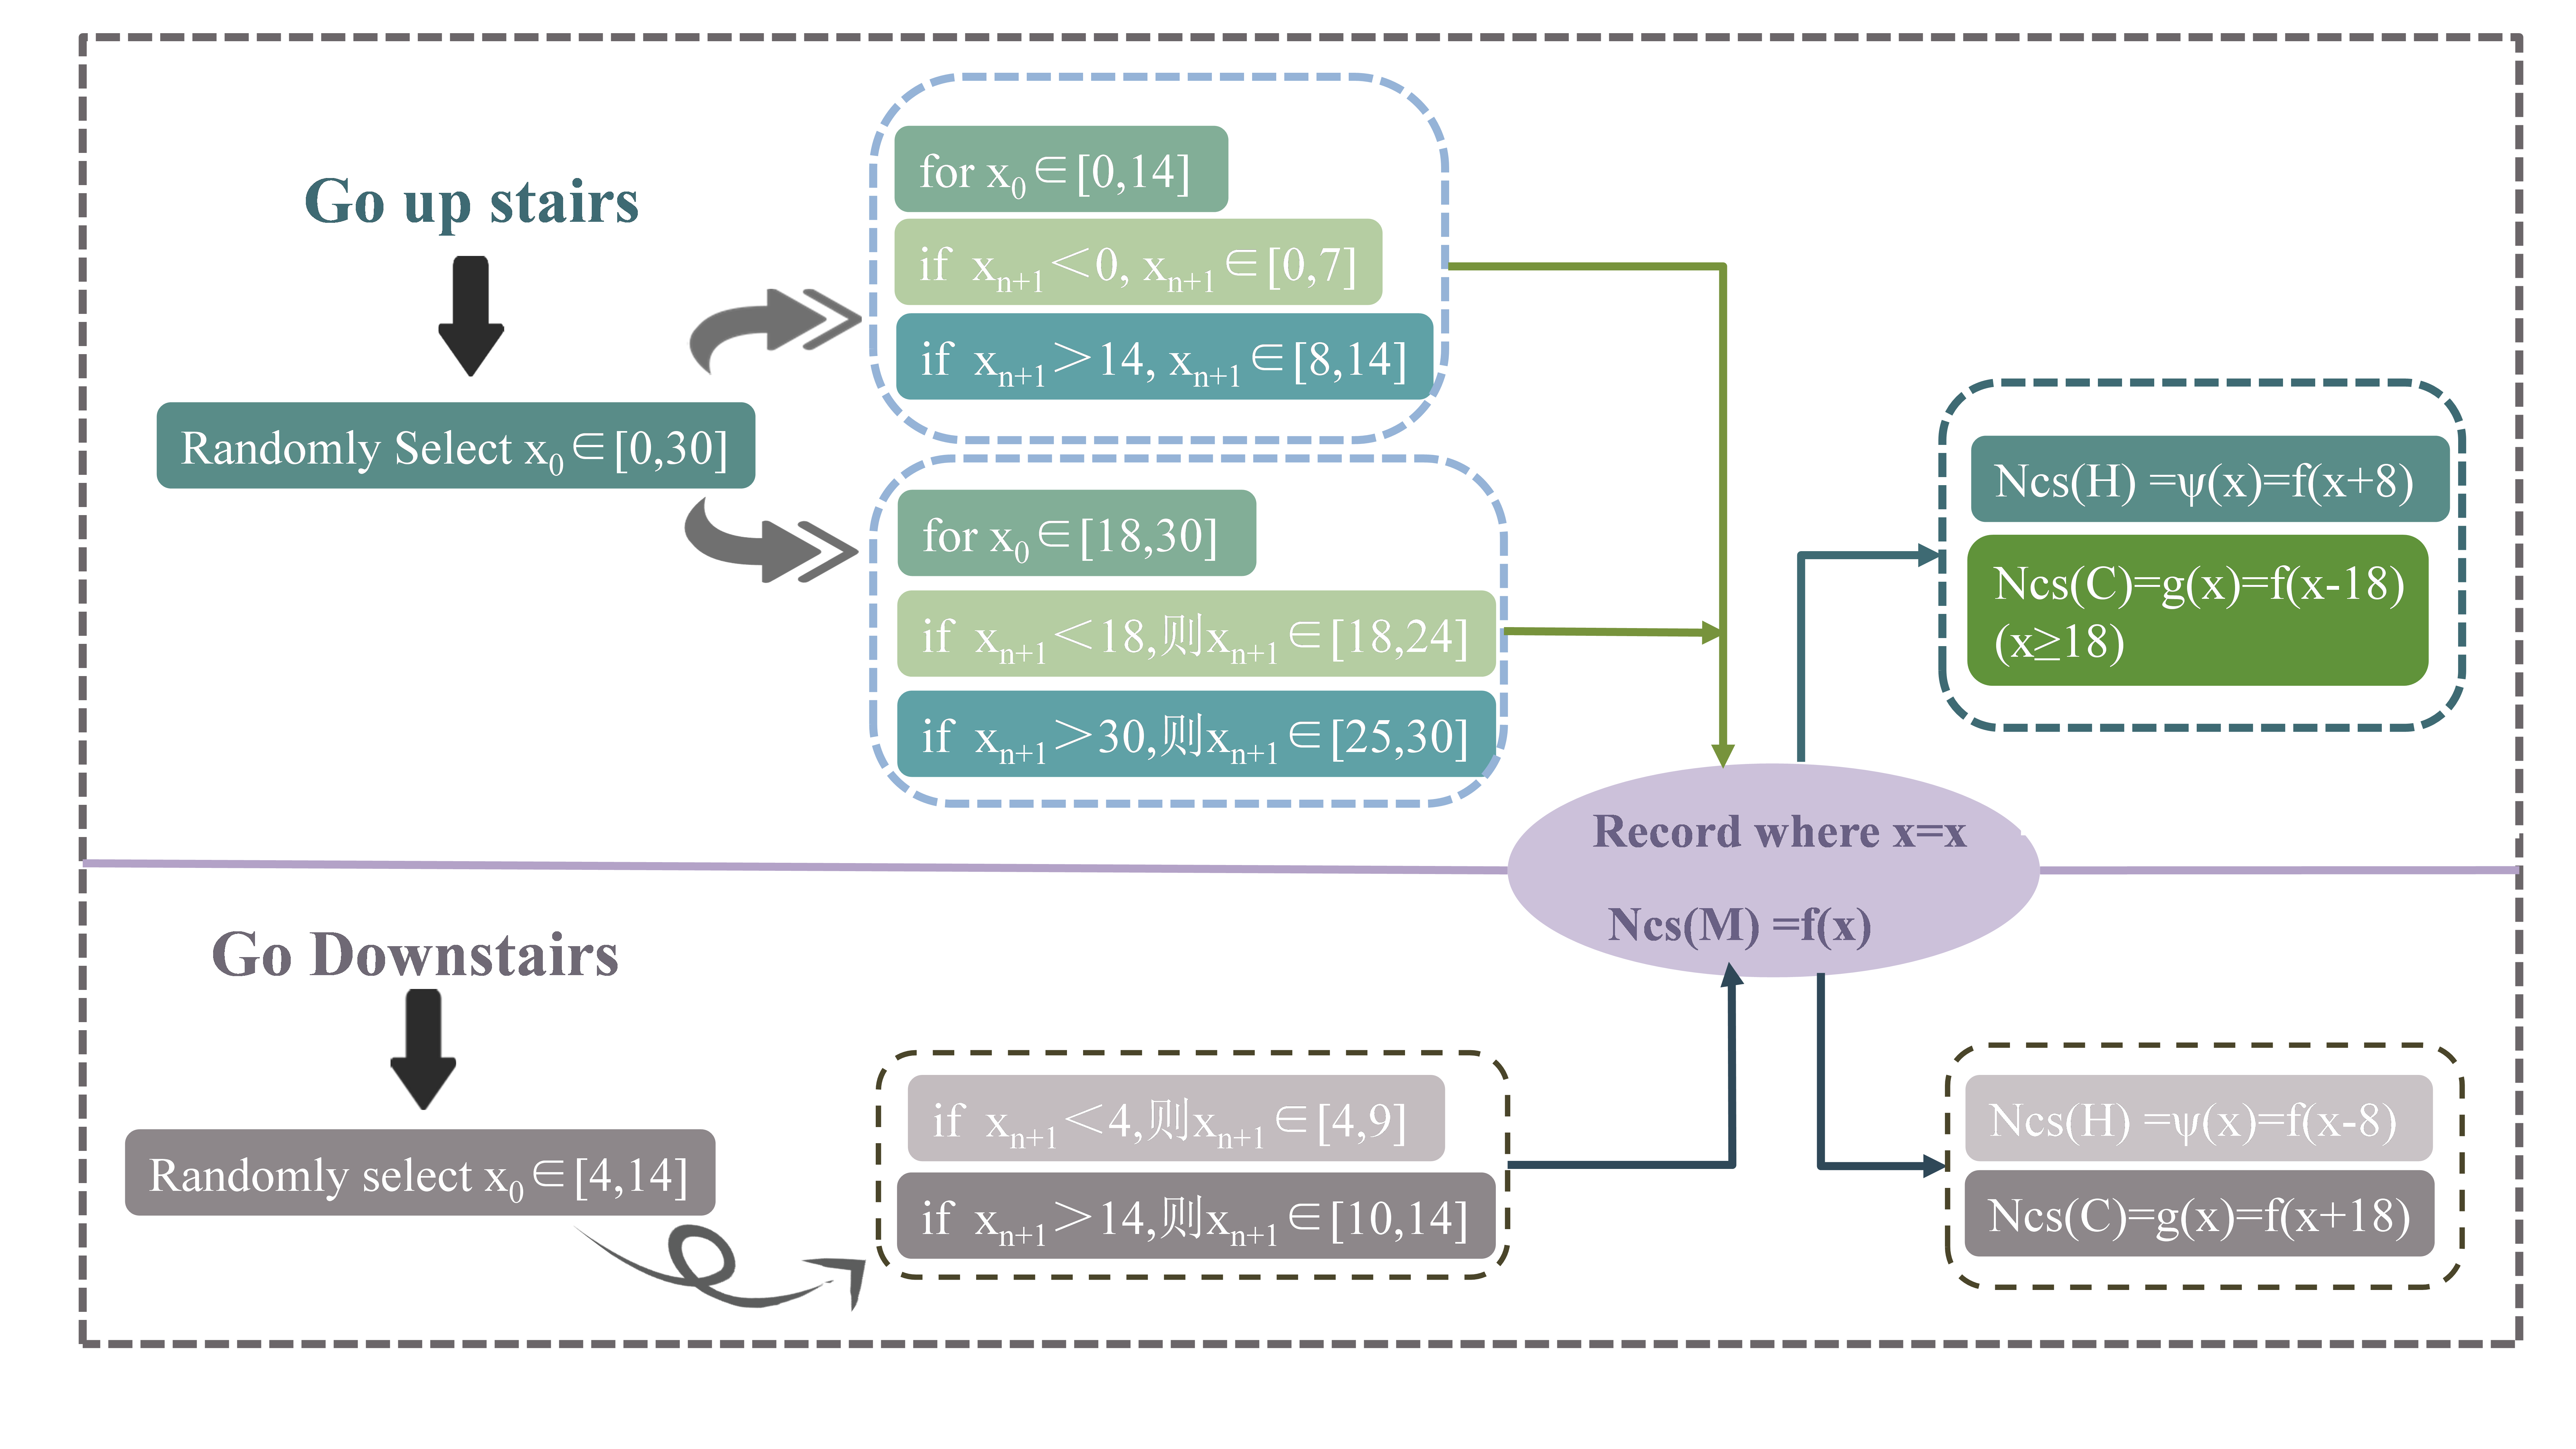
\includegraphics[width=12cm]{9-The flowchart for calculating the cumulative number of landing points.png}
    \caption{The flowchart for calculating the cumulative number of landing points} \label{fig:2}  % 标题与标签
    \end{figure}  % 图片结束
  
  
  After multiple iterations ,combining the coordinate relationships of the three main force regions, the model generates a distribution curves of the three main force-bearing areas of human feet
  \newpage
  
  \begin{figure}[h]  % 图片
    \small
    \centering  % 居中
    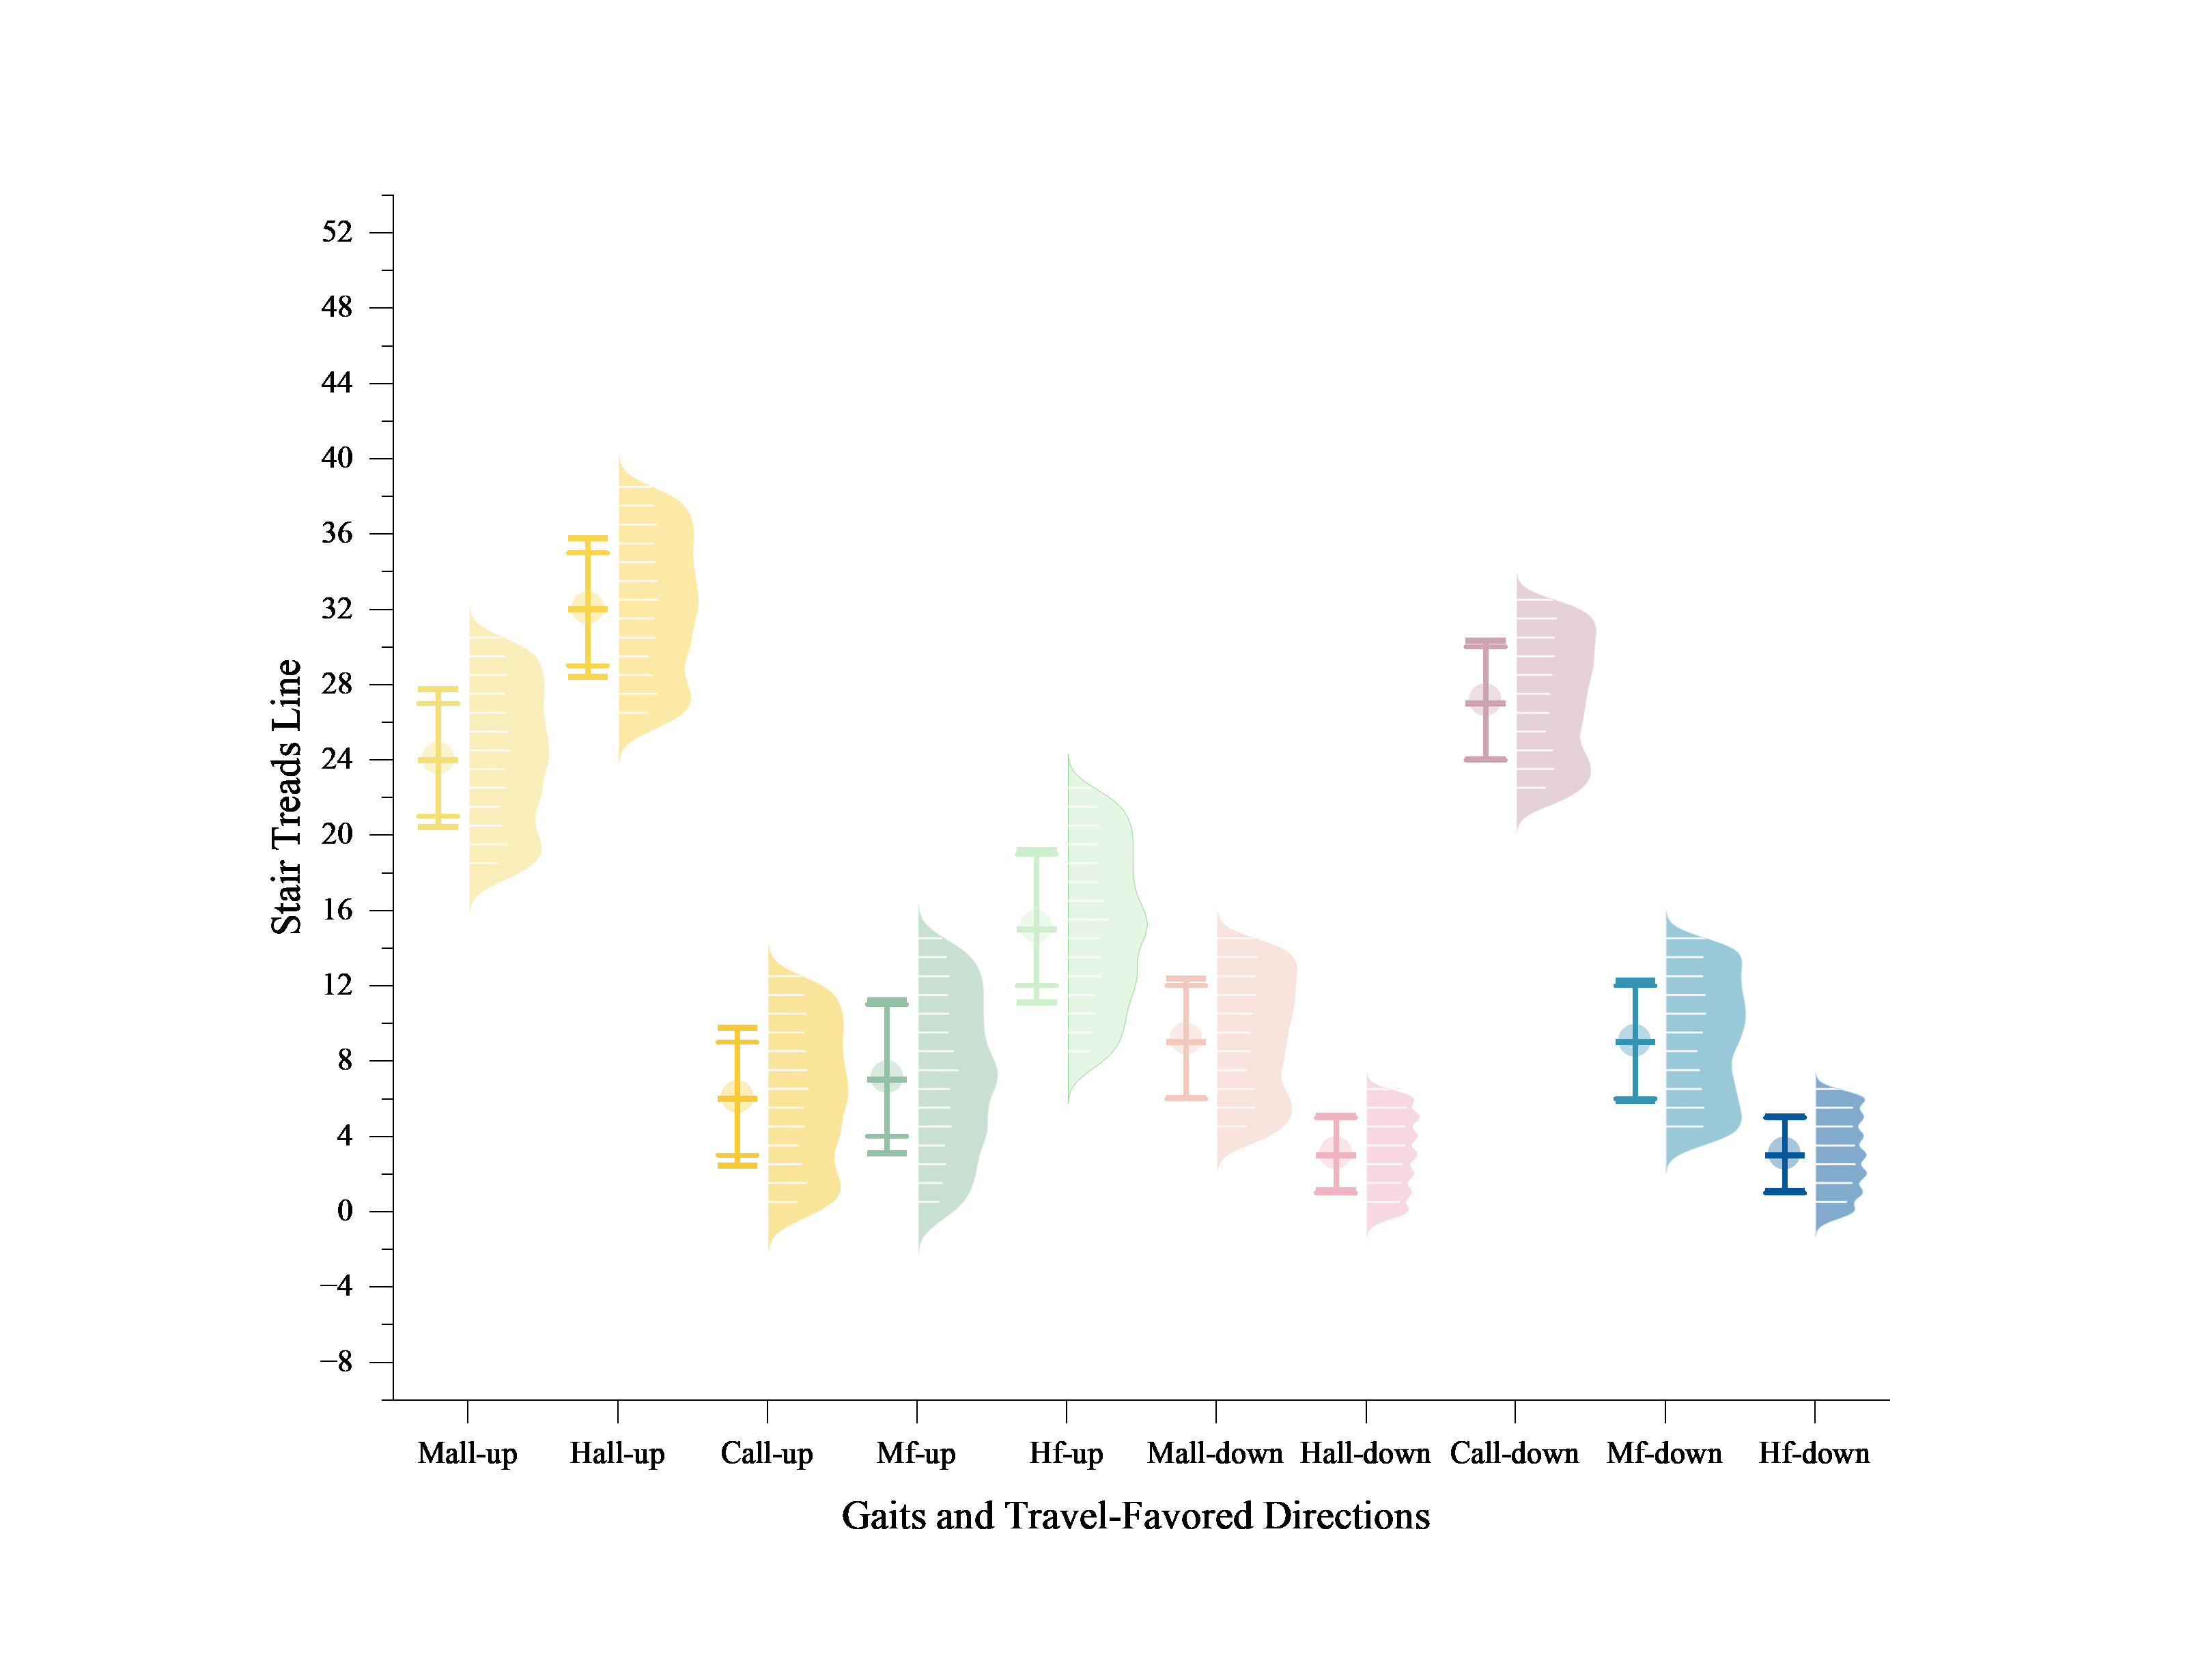
\includegraphics[width=12cm]{10-The Distribution of the Number of Landing Points of M,H and C.png}
    \caption{The Distribution of the Number of Landing Points of M,H and C} \label{fig:2}  % 标题与标签
    \end{figure}  % 图片结束
  
  
  \subsection{Conclusion}
  The Distribution of the Number of Landing Points of M, H and C has been obtained, laying the foundation for the derivation of the Staircase Section Worn Pit Profile Line.
  
 
  
\section{MESH Analysis Model}

\subsection{Wear depth analysis of a single step}
  \begin{itemize}[label=$\diamond$]
  
    \item \textbf{Full-foot Walking}
  Literature \cite{ WOS:000678697003082}provides proportional relationships between the forces exerted by the three main force regions of the foot when a person walks on stairs. These ratios reflect the magnitude of the forces exerted on the stairs by the different regions. The results were plotted as a trilinear diagram below:
  
  \begin{table}[h!]
    \centering
    \caption{Proportional Relationships Between Forces in Three Main Force Regions}
    \begin{tabular}{@{}lccc@{}}
    \toprule
    \textbf{Direction} & \(\frac{F_{G_h}}{G}\) & \(\frac{F_{G_m}}{G}\) & \(\frac{F_{G_c}}{G}\) \\ \midrule
    Up   & \( \frac{10}{23} \)  & \( \frac{41}{115} \) & \( \frac{24}{115} \) \\
    Down & \( \frac{40}{209} \) & \( \frac{50}{209} \) & \( \frac{29}{209} \) \\ \bottomrule
    \end{tabular}
    \end{table}

  Where\( G = 1624 \pm 19.2 \, \text{N} \) (from \cite{1})%%%%%%%%%%%%%%%%%%%%%%%%%%%%%%%%%%%%%%%%%%%%%%%%%%%%%%%%%%%%%%%%%%%%%%%%%%%%%%%%%%%%%%%%%%%%%%%%%%%%%%%%%%%%%%%%%%%%%%%%%%%%%%%%%%%%%%%%%%%%%%%%%%%%%%%%%%%%%%%%%%%%%%%%%%%%%%%%%%%%%%%%%%%%%%

  
  Where FGi is the vertical pressure exerted by region i on the stairs and G is the total vertical pressure.
  
  
  Assume that the wear volume can be approximated as a regular quadrangular pyramid, then based on its geometric characteristics, the wear depth in region m is calculated as:
  
  %%%%%%%%%%%%%%%%%%%%%%%%%%%%%%%%%%%%%%%%%%%%%%%%%%%%%%%%%%%%%%%%%%%
  Where Wm and \(S_m\) represent the wear volume and area of the m-th region, respectively.
  \item \textbf{Forefoot Walking}
  
  The wear analysis of forefoot walking is similar to that of full-foot walking, but the proportional distribution of forces is different from that of full-foot walking due to the fact that there are only two main force regions applying forces. In Fig. N, a trilinear diagram was plotted to show the relationship between the force distribution in the two regions. The depth of wear was calculated in the same way as for full-footed walking, with only the parameters adjusted.
  \end{itemize}

To study stair wear due to friction when a person walks, MESH analysis model is constrycted. A walkway width a person walks on stairs is at least equal to the average shoulder width (disregarding extreme crowding) and does not walk tightly against the edges of the stairs. 

On this basis, we divide the plane of the staircase into several walkways, each with a width approximately equal to the average shoulder width. Multiple walks cover almost the entire width of the stairs, with the excess width evenly distributed between the left and right sides of the stairs in the direction of travel.
\begin{itemize}[label=$\diamond$]
\item \textbf{Delineation of the target area of the stairs}
\end{itemize}

Combining the actual walking pattern, the force of human walking on stairs can be classified into the following four patterns:


%%%%%%%%%%%%%%%%%%%%(图)


\subsection{}

To analyze the effect of walking patterns on the stairs more accurately, the actual stepping area at the intersection of each step of the stairs and the walkway is defined as the target area. In the plan view of the stairs, the target areas are divided into four sub-areas, numbered 1, 2, 3, and 4, based on the functional characteristics of walking patterns(shown in Fig. 10).

\begin{figure}[h]  % 图片
  \small
  \centering  % 居中
  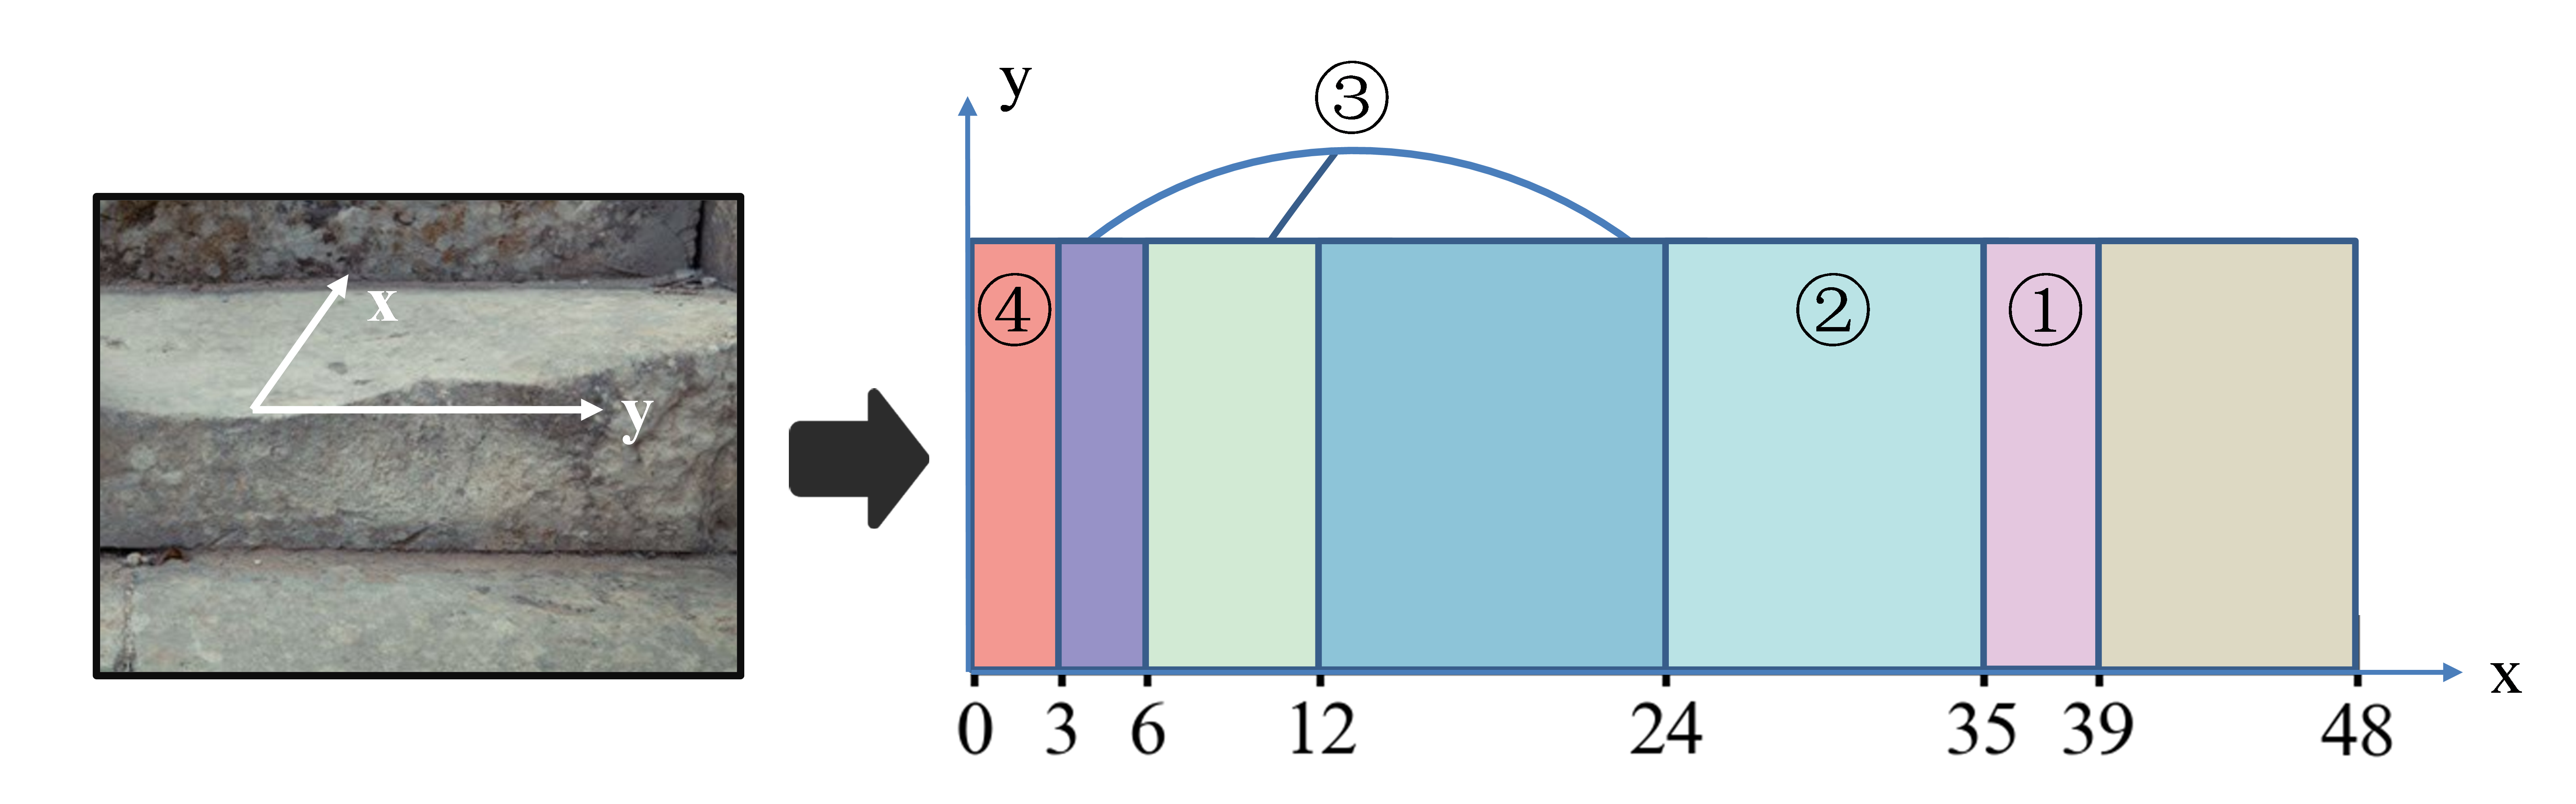
\includegraphics[width=10cm]{12-Explanation of the Division of the Pathways.png}
  \caption{Explanation of the Division of the Pathways} \label{fig:2}  % 标题与标签
  \end{figure}  % 图片结束


Sub-areas 1, 2, and 3: These areas correspond to the combined effects of different walking patterns, and their wears need to be analyzed separately according to the force characteristics of different patterns.

Sub-area 4: Located at the edge of the staircase, its influence is ignored in this study due to the large and rather small area affected by accidental factors.

With the above division, we clarify the force characteristics of different sub-regions by combining the four walking modes.

First, process the data measured by the archaeologists using the following formula:

\[ X_1 = CE_1 - Wr^{\frac{35 + 28}{2}} \cdot \left(k_A + k_B + k_C + k_D\right) \]

\[ X_2 = CE_2 - Wr^{\frac{24 + 34}{2}} \cdot \left(k_A + k_B + k_C + k_D\right) \]

\[ X_3 = CE_3 - Wr^{\frac{12 + 23}{2}} \cdot \left(k_A + k_B + k_C + k_D\right) \]

\[ X_4 = CE_4 - Wr^{\frac{6 + 11}{2}} \cdot \left(k_A + k_B + k_C + k_D\right) \]

\[ X_5 = CE_5 - Wr^{\frac{3 + 5}{2}} \cdot \left(k_A + k_B + k_C + k_D\right) \]

 Next, the force on each sub-region is quantitatively calculated using the relevant formulas:
 \begin{align}
  X_1 &= K_A \cdot A_{35 \to 38} - \alpha \\
  X_2 &= K_A \cdot A_{24 \to 24} + K_B \cdot B_{24 \to 34} - \alpha \\
  X_3^* &= K_A \cdot A_{12 \to 23} + K_C \cdot C_{12 \to 23} + K_D \cdot D_{12 \to 23} - \alpha \\
  X_3^{**} &= K_A \cdot A_{6 \to 11} + K_B \cdot B_{6 \to 11} + K_C \cdot C_{6 \to 11} + K_D \cdot D_{6 \to 11} - \alpha \\
  X_3^{***} &= K_A \cdot A_{3 \to 5} + K_B \cdot B_{3 \to 5} + K_C \cdot C_{3 \to 5} + K_D \cdot D_{3 \to 5} - \alpha
  \end{align}
  

Where $X_i$ represents the total depth of wear due to friction in sub-area i; $k$ refers to the number of people; $A_{i \to j}$ refers to the depth of friction due to friction at a time corresponding to the range of distance from the edge of the staircase from i to j; and $\alpha$ is the amount of wear in the target area due to environmental factors (e.g. temperature changes, humidity fluctuations, extreme weather, etc.).

The formulae for subregions 1, and 2 have been given above, and since there is no direct function to calculate $X_3$ for subregion 3, Probability-based fitting method is designed to calculate the total depth of wear due to friction. The pseudo code is as follows:

\renewcommand{\algorithmicrequire}{\textbf{Input:}}
\renewcommand{\algorithmicensure}{\textbf{Output:}}

\begin{algorithm}
\caption{Calculation of Material Correction Coefficients}
\textbf{Input:} $X_3, X_4, X_5, K_A, K_B, A, B, C, D, \alpha, \Phi(x)$\\
\textbf{Output:} $K_c, K_D$
\begin{algorithmic}
\State \textbf{for} $K_c \in \text{Range}(100, 100000)$ \textbf{do}
    \State \hspace{1em} $K_D = (X_5 - K_A A_{12\text{-}23} - K_c C_{12\text{-}23} - \alpha) / D_{12\text{-}23} $
    \State \hspace{1em} $X_{I_3} = K_A A_{3\text{-}5} + K_B B_{3\text{-}5} + K_c C_{3\text{-}5} + K_D D_{3\text{-}5} - \alpha$
    \State \hspace{1em} $X_{I_4} = K_A A_{6\text{-}11} + K_B B_{6\text{-}11} + K_c C_{6\text{-}11} + K_D D_{6\text{-}11} - \alpha$
    \State \hspace{1em} $\mathcal{E} = \Phi(X_{I_3} - X_3) - \Phi(-X_{I_3} - X_3)$
    \State \hspace{1em} $\mathcal{U} = \Phi(X_{I_4} - X_4) - \Phi(-X_{I_4} - X_4)$
    \State \hspace{1em} $\text{Result}[i] = \left[ \frac{\mathcal{E}}{\mathcal{U}}, K_c, K_D \right]$
    \State \hspace{1em} $i = i + 1$
\State \textbf{end}
\State Find the maximum $\text{Result}[n][1]$
\State \textbf{Output:} $K_c = \text{Result}[n][2], K_D = \text{Result}[n][3]$
\end{algorithmic}
\end{algorithm}

\section{Conclusion of Basic Predictions}



Initially, we assume that when only one person is walking on the stairs, the walkway selection for each step remains consistent, meaning they will walk along the same walkway throughout. Based on the results obtained from the pseudocode, we can derive the total number of people on each walkway as follows:

\[ K_i = K_{Ai} + K_{Bi} + K_{Ci} + K_{Di} \]

Using this expression, we can calculate the total number of people on each path, which is then visually represented using a bar chart (as shown in Figure n).

After calculating the total number of people on each walkway, we further sum these values to obtain the total number of people using the stairs, expressed as:

\[ K_{\text{total}} = \sum_{i=1}^n K_i \]


\subsection{Question A: Usage frequency}

The question of "How often were the stairs used?" is quantified as the average usage frequency of the stairs over the total usage time, with the calculation formula as follows:

\[ \text{usage frequency} = \frac{K_{\text{total}}}{\text{total usage time}} \]

On this basis, the average time interval between uses of the stairs is obtained as .......

\subsection{Question B: Directional preference}

The total number of people descending the stairs can be expressed as:

\[ K_{\text{downstairs}} = K_B + K_D \]

The total number of people ascending the stairs can be expressed as:

\[ K_{\text{upstairs}} = K_A + K_C \]

By comparing the total numbers of ascending and descending, We can draw the following conclusions regarding the direction of travel favored by the people using the stairs:

\begin{itemize} 

\item If $K_{\text{upstairs}}>K_{\text{downstairs}}$, it indicates that the travel direction favored by the people using the stairs is \textbf{ascending}. %%%%

\item If $K_{\text{upstairs}}<K_{\text{downstairs}}$, it indicates that the travel direction favored by the people using the stairs is \textbf{descending}. %%%%%

\end{itemize}


\subsection{Question C: Usage mode}
The Z-scores formula can be used to determine outliers in the data. When the Zi corresponding to the ith data in a data set satisfies the condition Zi>3.5\cite{curtis2016mystery},  it can be considered that this data point is a peak. The Z-scores formula is as follows:

\[ Z_i = \frac{K_i - \bar{K}}{\sqrt{\text{Var}(K)}} \]

Where Var($K$) refers to the variance of the number of people on walkways and represents the mean value of the number of people on walkways.


%%%%%%%%%%%%%%%%%%%%%%%%%%%%%%%%%%%%%%%%%%%%%%%%%5

If a peak exists, it indicates that the number of people on a certain walkway is significantly higher than on other paths, suggesting that people tend to walk in a line;

If there is no peak, it indicates that the distribution of people across walkways is relatively uniform, suggesting that people prefer to walk side by side.

\section{Guidance Based on Stairwell Usage}
\subsection{Question D: The fit consistency}
When evaluating the model fit with $\varepsilon +\eta$ , if the confidence is greater than 95\% (i.e. less than 1.9), the model is considered to have a good fit with the actual data. Additionally, if the confidence is less than 0.95, the fit is considered excellent.
\subsection{Question E: Age of the stair }

Based on the wear data shown in (Figure x), the wear in the 39-48 range is primarily influenced by environmental factors, exhibiting a Micro-weathering effect, and it is assumed that no significant wear is caused to the stairs.

\textbf{!!WARNING Figure x is a placeholder, please replace it with the actual figure number WARNING!!}

On this basis, using the principles of probability theory, we can assume that the wear amount of the stairs caused each year follows a Gaussian distribution.

The total wear rate of the stairs is determined by both the average annual wear rate and the time (i.e. the number of years since construction), and their relationship is expressed as:

\[R_{\text{total}} = R_{\text{year}} \cdot T \]

Where $R_{\text{total}}$​ represents the total wear amount, $R_{\text{daily}}$​ is the annual wear amount, and T refers to the time span, which is the total number of years since the stairs were constructed.

Since division operations do not alter the distribution pattern of a Gaussian distribution, the estimated value of the construction year of the stairs also follows a Gaussian distribution. Therefore, we can further calculate the probability of the time period provided by the archaeologist within this estimated Gaussian distribution. The higher the probability, the more reliable the estimated value.

\subsection{Question F: Repairs and renovation}

The primary repair method for building materials is crack reinforcement using polymer materials\cite{YTLX200401034}. Steel plate bonding is also commonly used to strengthen flexural or tensile members (e.g. stair platform beams, slabs, and treads) under normal working and static loads. Another option is wrapping original staircase components with steel plates for protection.

For visible repairs or renovations, their presence can usually be confirmed by direct observation. However, for polymer reinforcement methods not easily visible, we designed the following detection approach:

First, we calculate the difference between the original depth data of surface depressions and the optimized depth data from the result of pseudo-code, identifying points with significant positive differences as abnormal depressions, which may indicate repairs.

Next, we conduct secondary sampling on the treads with abnormal depression points, increasing the sampling density to 300 samples per square meter. We repeat the abnormal point analysis on the new data. If the abnormal points show circular or strip-shaped clustering (as seen in Figure 11), we preliminarily conclude that the area may have been repaired with polymer reinforcement methods.
\begin{figure}[h]  % 图片
  \small
  \centering  % 居中
  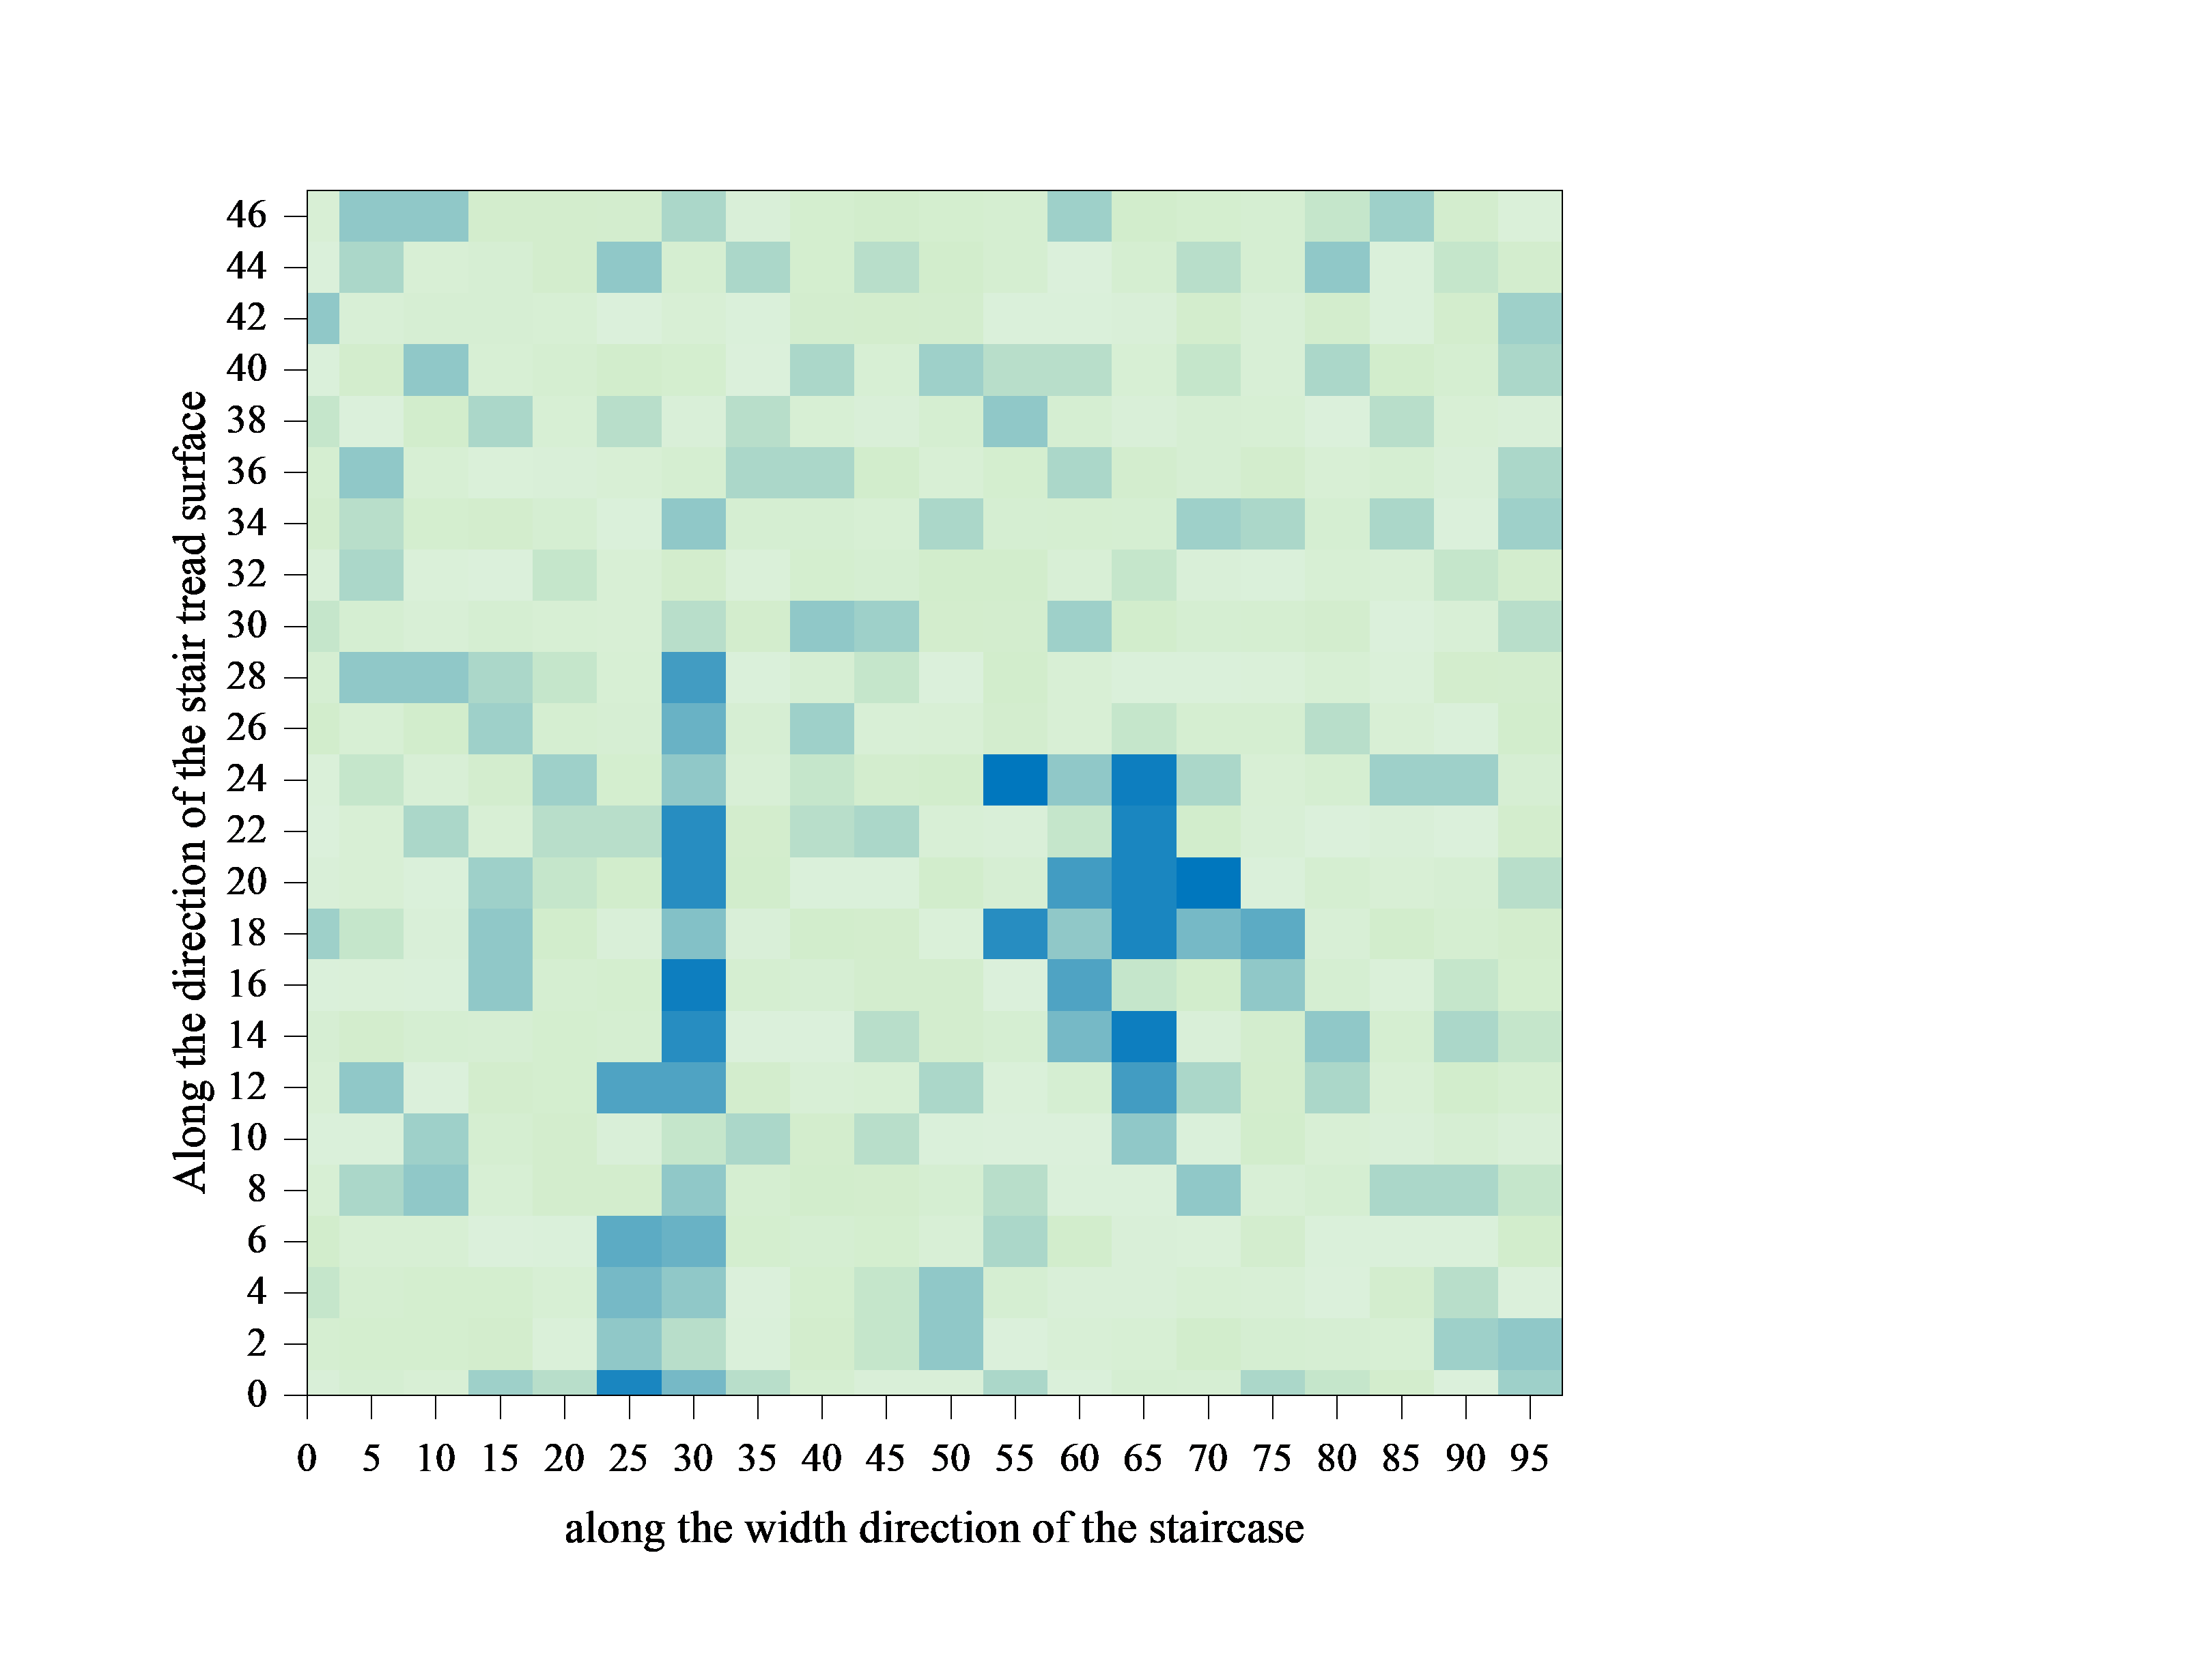
\includegraphics[width=11cm]{13-Illustrative cluster diagram of the renovated areas.png}
  \caption{Illustrative cluster diagram of the renovated areas} \label{fig:2}  % 标题与标签
  \end{figure}  % 图片结束



To further verify the use of polymer materials for reinforcement, we employ the Torrent Permeability Test Method to measure the air permeability of the building material\cite{sena2015non}. Polymer materials typically exhibit strong adhesion, no powder residues, water resistance, and polishability. However, their air permeability differs significantly from that of the base stone material. By comparing air permeability values, we can further confirm the presence and extent of repaired regions.

When further analyzing areas with abnormal air permeability, we perform water absorption tests on the associated staircase treads. The specific method is as follows:

To further study areas with abnormal air permeability, we performed water absorption tests on the associated staircase treads. The specific steps are as follows:

\begin{itemize}[label=$\diamond$]
\item \textbf{Testing Procedure}

1.Attach cobalt chloride test paper, fully saturated with water and turned pink, to both the clustered abnormal points and the normal areas of the staircase treads.

2.Cover the test paper with appropriately sized covers to prevent water evaporation.

3.Use a d345 camera to continuously monitor and record the color change of the test paper.


\item \textbf{Analysis of Test Results}


Cobalt chloride test paper turns blue upon water absorption. By monitoring the rate at which the paper turns blue, we can assess the water absorption capacity of different areas of the stone material.
If the test paper in the clustered abnormal points turns blue at a delayed rate, it indicates poor water absorption capacity in that area, further supporting the conclusion that polymer reinforcement has been applied.
Finally, by combining the test results with the surface water permeability characteristics of the material and comparing the water absorption differences 
between the clustered abnormal points and normal areas, the presence and spatial distribution of polymer material repairs can be further confirmed.

Through the above multi-level detection method, not only can the presence of repairs or renovations be scientifically determined, but the repaired areas can also be accurately identified.
\end{itemize}
\subsection{Question G: Consistency of mechanical parameters}

To determine whether the source of the target material aligns with the archaeologist's hypothesis, we recommend sampling from what the archaeologist believes to be the original source and conducting destructive mechanical experiments to obtain precise material parameters. These experimentally obtained parameters are then used to replace the tabulated values and are re-integrated into the Step Load Interaction Model to derive the optimal fitting result. Finally, this result is compared to the fitting result obtained using the tabulated parameters, with the coefficient of determination $R^2$ used as the evaluation criterion.


Goodness-of-fit calculation formula:


\[R^2 = \frac{\text{SSR}}{\text{SST}} = 1 - \frac{\text{SSE}}{\text{SST}}, \quad 0 \leq R^2 \leq 1 \]

\begin{itemize} 

\item The sum of Squares for Error (SSE): The sum of squared differences between the actual values and predicted values, reflecting the magnitude of errors. 

\item The sum of Squares for Regression (SSR): The sum of squared differences between the predicted values and the mean of the actual values, representing the variation explained by the model. 

\item The total Sum of Squares (SST): The sum of squared differences between the actual values and their mean, equivalent to the total variation. The relationship satisfies: 
\end{itemize}



\[\text{SST} = \text{SSE} + \text{SSR}\]

$R^2$ represents the proportion of the total variation that can be explained by the model. The closer the $R^2$ value is to 1, the higher the consistency of the model. The $R^2$ value can be used to evaluate the match between the archaeologist's hypothesized material source and the actual results. When $R^2$ exceeds 0.8, it indicates that the source of the target material is consistent with the archaeologist's hypothesis.


\subsection{Question H: Number of people and time scale}


\textbf{1.Number of Users in a Typical Day for Staircase }


In ... (referenced analysis), we have already obtained the total number of users during the operational period of the staircase. Assuming that the number of people using the stairs per day remains constant during this period, the number of people using the stairs in a typical day can be expressed as:

\[\text{Number of Users in a Typical Day} = \frac{\text{Total Number of Users}}{\text{Total Days of Usage}}\]

\textbf{2.Short-Time High Traffic or Long-Time Low Traffic}


Fatigue strength is significantly influenced by loading frequency, defined as the frequency at which force is applied to the
material\cite{Yokobori1976}\cite{Takezono1980}\cite{HeimbachHeimbach+1970+377+380}. Higher loading frequency accelerates the formation of micro-cracks within the material, which can rapidly propagate in a short
period\cite{ SJESAC88A958454EEE1CD4ED092FB8A0E8F8}.\cite{ SJESF46245B4D88236414B6977C781CEC048}, ultimately leading to fracture. This indicates that higher loading frequencies directly increase the probability of fracture by expediting crack propagation. Consequently, when a large number of people use the staircase within a short period, the increased loading frequency makes the formation and propagation of cracks within the staircase more likely, thereby increasing the risk of fracture.

Additionally, due to abrupt geometric transitions, the outer edges of staircases often exhibit stress concentration, which further accelerates fatigue damage. This stress concentration makes cracks more likely to propagate, ultimately resulting in material fracture. Observations of real structures corroborate this phenomenon, as cracks are predominantly concentrated along the outer edges of staircases, confirming the role of stress concentration.

In summary, when a large number of people use the staircase within a short period, the increased loading frequency and stress concentration at the outer edges are primary contributors to crack formation and propagation, ultimately leading to material damage and even fracture.

To quantify this effect, we evaluate the depression depth $X_6$ in the 0–3 step region of the staircase using the following equation:


\[\text{LFP} = X_6 - k_A A_{0-3} - k_B B_{0-3} - k_C C_{0-3} - k_D D_{0-3}\]


In cases of significant normal wear, the fracture risk in this region increases notably. 

To assess the relationship between $X_6$ and the loading frequency parameter \text{LFP}, a Mann-Whitney U test is used. Since $X_6$ and $X_6$ + \text{LFP} share similar data distributions and do not require identical distributions, the test is applied to determine whether $X_6$ + \text{LFP} is significantly greater than $X_6$. The hypotheses are as follows:


\begin{itemize} 
\item Null Hypothesis (H\(_0\)): \(X_6 + \text{LFP}\) is not significantly greater than \(X_6\). 
\item Alternative Hypothesis (H\(_1\)): \(X_6 + \text{LFP}\) is significantly greater than \(X_6\). 
\end{itemize}

The U statistic is calculated as follows:

$$U = n^2 + \frac{n}{2}(n + 1) - R(X_6)$$

Here, R represents the calculation of the sum of ranks.

At a significance level of \(\alpha = 0.05\), the rejection region is \(U < 8\). The decision criteria are:
\begin{itemize} 

\item If U < 8, the alternative hypothesis $H_1$ is accepted, indicating material loss at the staircase edges caused by fractures.

\item If \(U \geq 8\), the null hypothesis $H_0$ is accepted, suggesting that material loss at the staircase edges is primarily due to normal wear and bending, with no additional fractures.

\end{itemize}

Based on the Mann-Whitney U test results, the following conclusions can be drawn:


\begin{itemize} 
\item If a significant difference exists between \( X_6 \) and \( \text{LFP} \), it indicates that material loss at the staircase edges is not solely caused by normal wear and bending but is also due to a large number of people using the staircase in a short time. 
\item If no significant difference exists between \( X_6 \) and \( \text{LFP} \), it indicates that a small number of people use the stairs over an extended time. 
\end{itemize}

By integrating the Mann-Whitney U test results with the theoretical analysis, this method enables a reasonable determination of whether the staircase was used by a large number of people over a short time or by a small number of people over a long time.


\section{Sensitivity Analysis}

Due to the orientation of a person's stance during walking, which is taken into account by the model, the preferences for going up or down are not fixed. Any change in parameters may lead to a different profile of the worn pit in the staircase section. Consequently, by changing a certain parameter and solving the model, the sensitivity of the model can be verified.

Maintaining the total number of people unchanged, by changing the ratio of $K_{\text{upstairs}}$ to $K_{\text{downstairs}}$ and simulating, the shapes of the depressions under different parameters can be obtained(Fig.12).
As can be seen from the Fig.12 with the decrease of the proportion of people walking up stairs, the depth of the depression near the edge increases, while the depth of the depression in the area far from the edge decreases. The change in the ratio of the number has a significant impact on the result, indicating that the model is highly sensitive. Therefore, the fitting of K is feasible and accurate.

\begin{figure}[h]  % 图片
  \small
  \centering  % 居中
  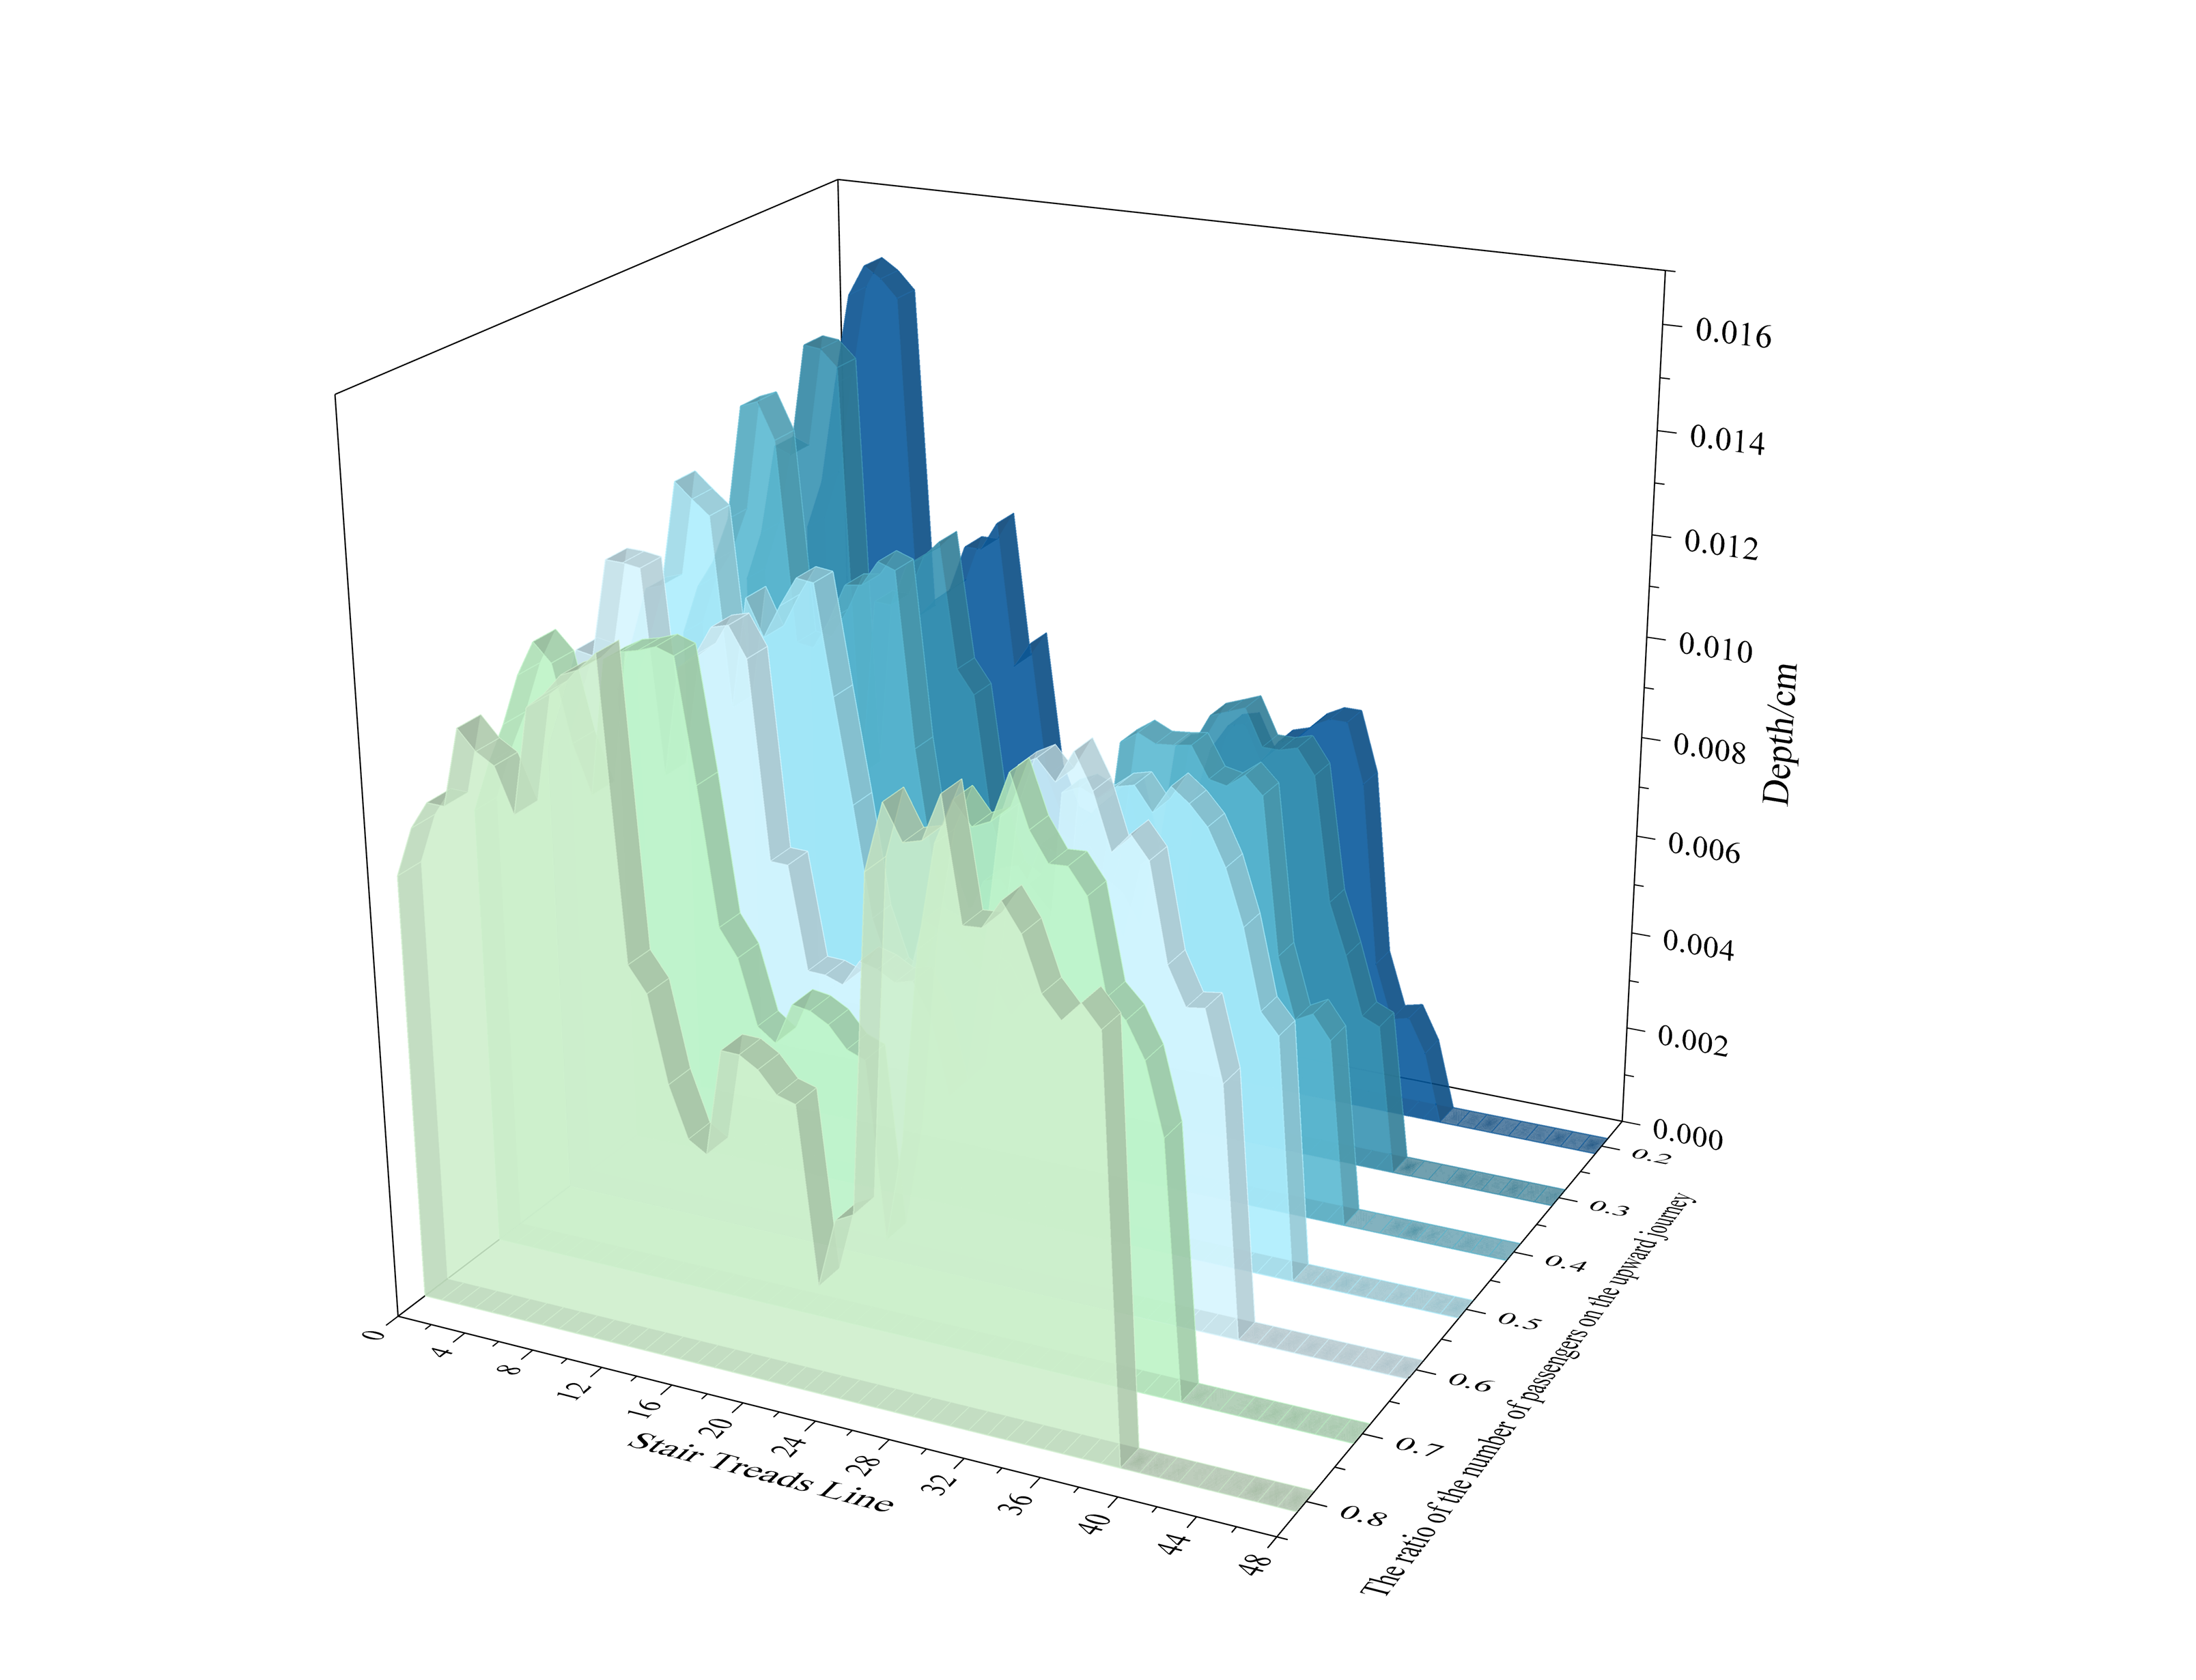
\includegraphics[width=11cm]{14-Staircase section Worn Pit Profile Line varies with the ratio of the number of passengers on the upward journey..png}
  \caption{Staircase section Worn Pit Profile Line varies with the ratio of the number of passengers on the upward journey} \label{fig:2}  % 标题与标签
  \end{figure}  % 图片结束
\section{ Evaluation of Strengths and Weaknesses}%或者做成 Model Evaluation and Further Discussion多一个Model Extension小部分
\subsection{Strengths}
\subsection{Weaknesses and Further Improvements}
\section{Conclusion}

\newpage

\renewcommand{\refname}{References} % 确保标题显示为 References
\addcontentsline{toc}{section}{References} % 手动加入目录
\patchcmd{\thebibliography}{\section*}{\section*}{}{} % 移除编号
\nocite{*}

\bibliographystyle{ieeetr} % 可选格式:plain、ieeetr、apalike 等
\bibliography{References}
\begin{appendices}  % 附录

\end{appendices}  % 附录结束
\end{document}